% ===================================================
% CHƯƠNG 2: MÔ HÌNH ĐỘNG VÀ THIẾT KẾ GIAO DIỆN UI/UX (SUBMISSION #2)
% Nguồn: app/prototype/, docs/diagrams/02_Sequence_Diagram/, 03_Activity_Diagram/, 04_Statechart_Diagram/
% Slide tham chiếu: 06_Ch6 System Modeling_2025.pdf (Interaction & Behavioral Models)
% ===================================================
\section{Mô hình Động và Thiết kế Giao diện (Dynamic Models and UI Design)}

\subsection{Thiết kế Giao diện UI (UI Design: Mockup -- 26 Màn hình)}

\subsubsection*{Triết lý Thiết kế: Hai Luồng Nghiệp vụ và Ba Giao diện Độc lập}
Bản mẫu giao diện (\textit{UI Mockup}) được xây dựng bằng HTML5, CSS3 và JavaScript thuần tại \texttt{app/prototype/} (\texttt{index.html}, \texttt{app.js}, \texttt{styles.css}), sử dụng bảng màu Primary Navy \texttt{\#152584}, Accent Cyan \texttt{\#00B8D6} và nền \texttt{\#F2F5F9}. Hệ thống tách biệt ba giao diện theo thẩm quyền tác nghiệp (nút chuyển trên thanh công cụ của \texttt{index.html} chỉ phục vụ duyệt thiết kế ngoại tuyến, không phải cơ chế đổi quyền trên máy chủ):
\begin{enumerate}[leftmargin=*,nosep]
    \item \textbf{Mobile User App (bản mẫu trong \texttt{index.html}):} Trình bày luồng người dùng cuối thực hiện \texttt{UC01--UC07} trên thiết bị di động (không cung cấp giao diện Web PC đặt xe cho \texttt{User}). Ở sản phẩm chạy thật, luồng này được hiện thực bằng ứng dụng Native Android (\texttt{android/}) và client Flutter (\texttt{app/flutter\_mobile/}).
    \item \textbf{Mobile Operator App (\texttt{/operator-app.html}):} Giao diện thẻ di động tối ưu thao tác một tay cho \texttt{Operator} hiện trường qua thanh điều hướng dưới và menu \texttt{\#op-menu}; khi chạy qua máy chủ Express sẽ chuyển hướng tới \texttt{live.html?\allowbreak experience=operator-app}.
    \item \textbf{Desktop Operator Web Dashboard (\texttt{/operator-web.html}):} Bảng điều khiển trên máy tính với thanh bên, thẻ KPI, bản đồ MapLibre và bảng dữ liệu phân tích \textit{What-if}; chuyển hướng tới \texttt{live.html?\allowbreak experience=operator-web}.
\end{enumerate}

\Cref{fig:ui-user-board} trình bày chuỗi màn hình thiết kế của phân hệ Người dùng (từ tìm Hub, xem xe, đặt giữ đến đỗ và sạc xe cá nhân), còn \Cref{fig:ui-operator-board} tổng hợp các màn hình của phân hệ Vận hành trên cả giao diện di động và desktop (bản xuất đầy đủ gồm 14 trang A4 Landscape trong \texttt{app/prototype/UI-UX.pdf}).

\begin{figure}[H]
    \centering
    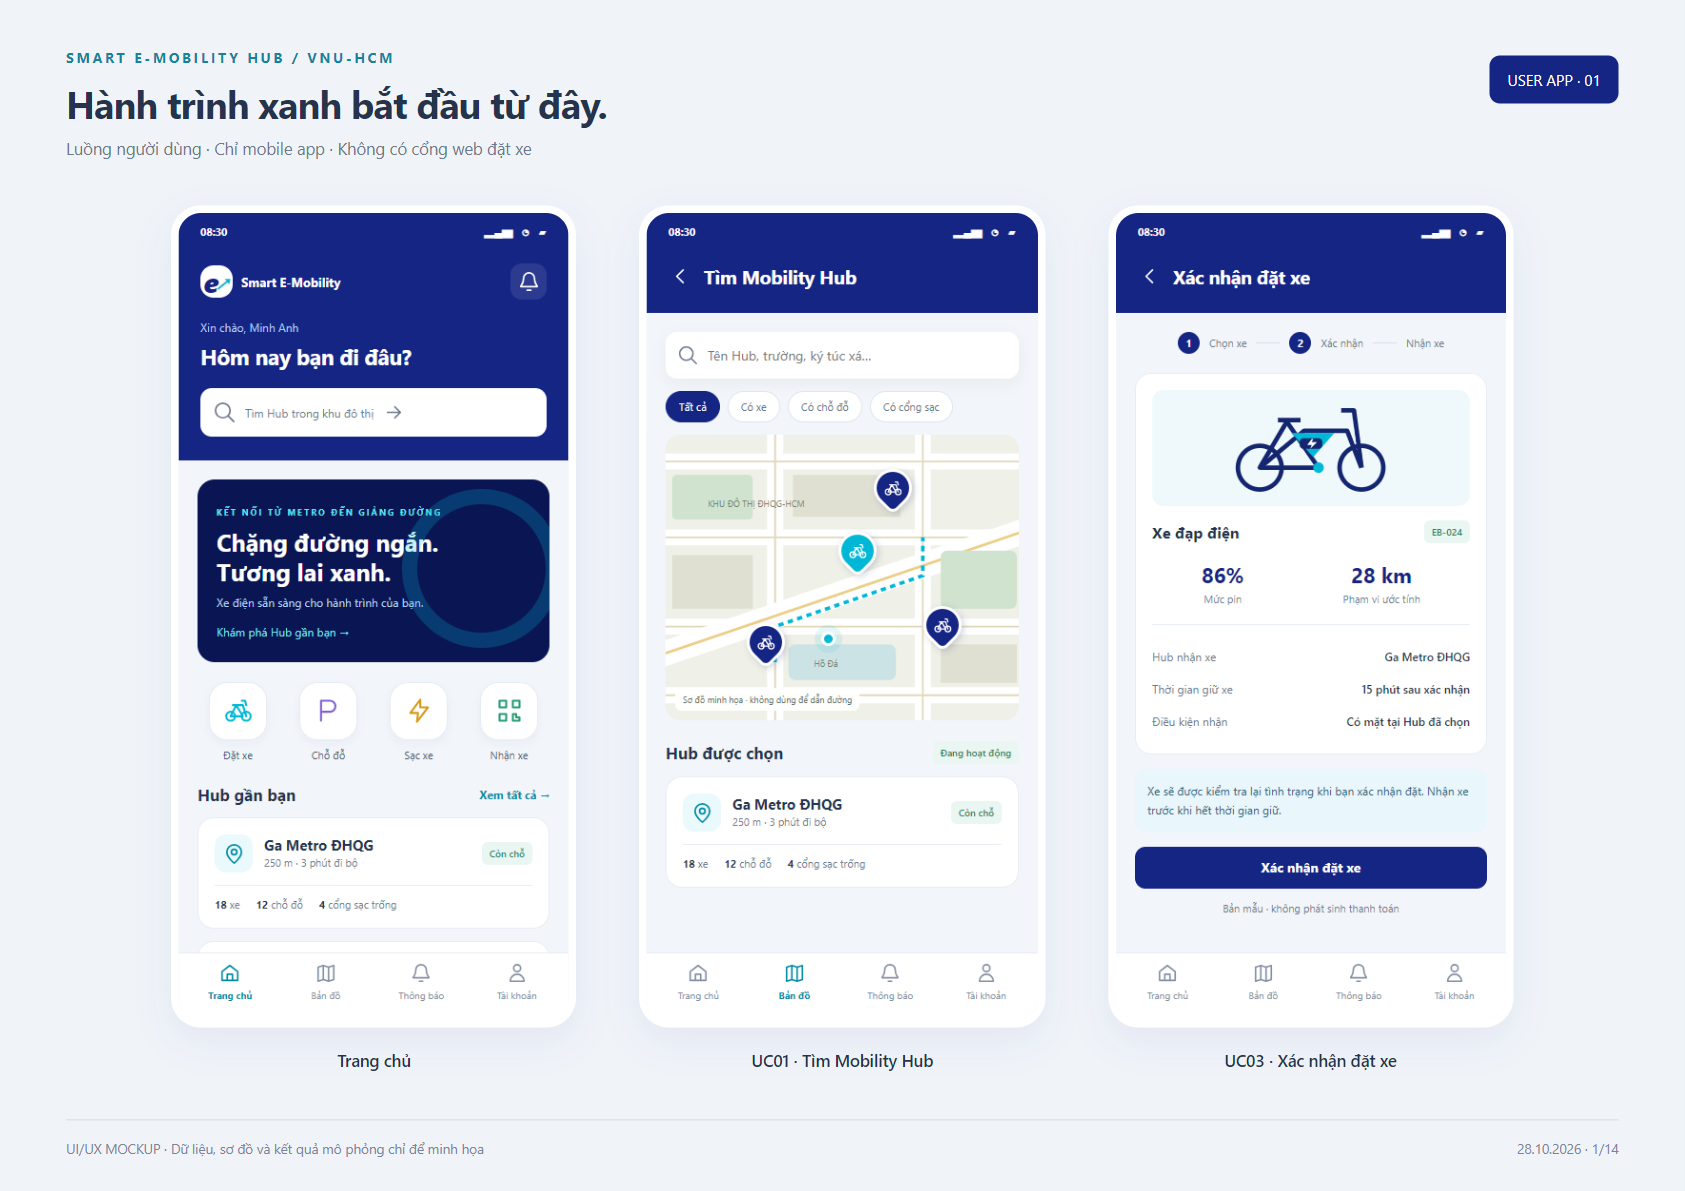
\includegraphics[width=0.95\textwidth]{../../../app/prototype/design-board.png}
    % Nguồn ảnh: app/prototype/design-board.png
    \caption{Tổng quan giao diện Mobile Người dùng (\texttt{app/prototype/design-board.png})}
    \label{fig:ui-user-board}
\end{figure}

\begin{figure}[H]
    \centering
    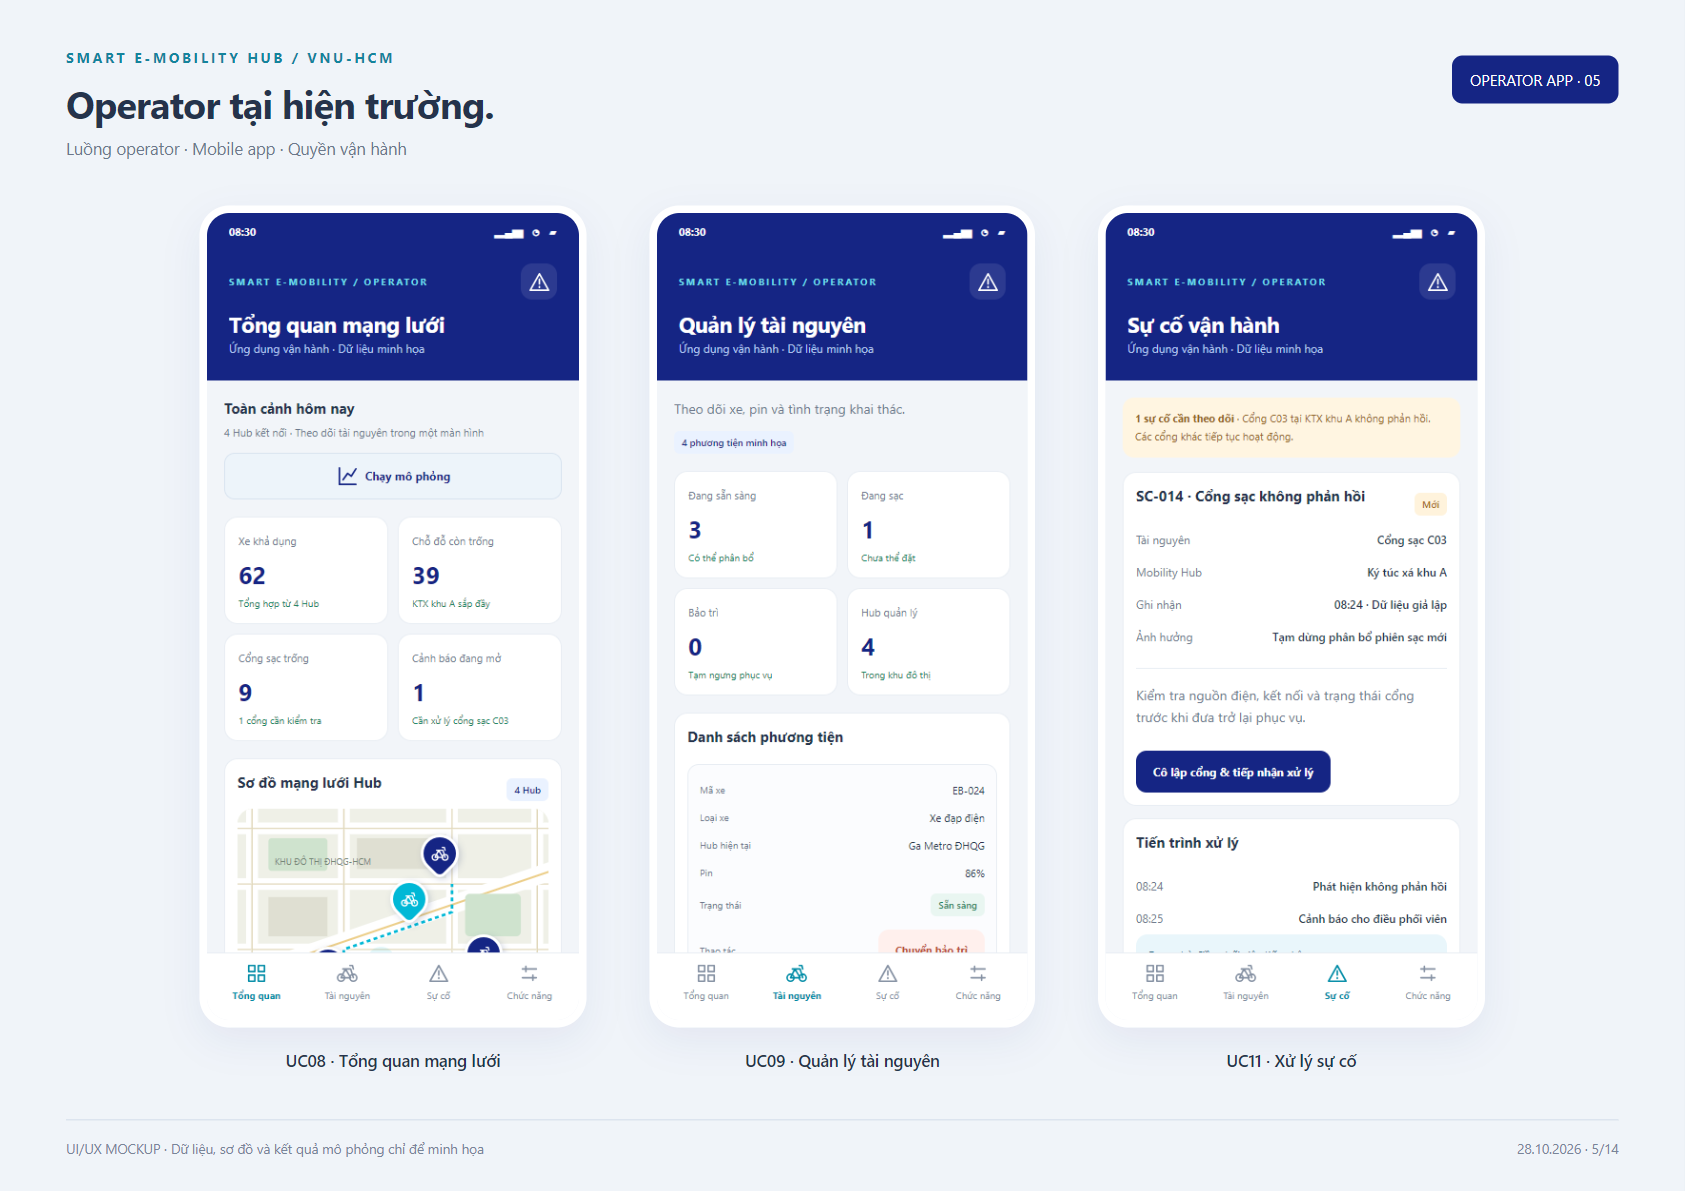
\includegraphics[width=0.95\textwidth]{../../../app/prototype/operator-app-board.png}
    % Nguồn ảnh: app/prototype/operator-app-board.png
    \caption[Tổng quan giao diện Mobile và Web Vận hành]{Tổng quan giao diện Mobile và Web Vận hành (\texttt{app/prototype/operator-app-board.png})}
    \label{fig:ui-operator-board}
\end{figure}

\subsubsection*{Ánh xạ 14 Use Cases sang 26 Màn hình và Kiểm định Playwright}
\Cref{tab:ui-26-screens} đối chiếu toàn bộ 26 tệp ảnh giao diện tại \texttt{app/prototype/screens/} với mã Use Case tương ứng. Bộ kiểm thử tự động \texttt{app/prototype/verify.cjs} chạy trên Playwright xác nhận 26/26 màn hình hiển thị không lỗi JavaScript (\textit{console error}) và không tràn bố cục ngang trên cả Mobile (\texttt{390px}) và Desktop (\texttt{1280px}), kết quả lưu tại \texttt{app/prototype/verification.json} (\texttt{passed: true}).

\begin{longtable}{>{\centering\arraybackslash}p{1.4cm} >{\raggedright\arraybackslash}p{3.9cm} >{\centering\arraybackslash}p{2.1cm} >{\raggedright\arraybackslash}p{6.8cm}}
\caption{Bảng ánh xạ 14 Use Cases sang 26 màn hình giao diện (\texttt{app/prototype/screens/})} \label{tab:ui-26-screens} \\
\toprule
\textbf{Mã UC} & \textbf{Nhóm nghiệp vụ} & \textbf{Nền tảng} & \textbf{Màn hình và tệp ảnh (\texttt{screens/})} \\
\midrule
\endfirsthead
\toprule
\textbf{Mã UC} & \textbf{Nhóm nghiệp vụ} & \textbf{Nền tảng} & \textbf{Màn hình và tệp ảnh (\texttt{screens/})} \\
\midrule
\endhead
\bottomrule
\endfoot
-- & Trang chủ, Thông báo, Tài khoản & Mobile User & \texttt{home.png}, \texttt{notifications.png}, \texttt{account.png} \\
\texttt{UC01} & Tìm kiếm Hub di chuyển & Mobile User & \texttt{map.png} (\texttt{\#map}) \\
\texttt{UC02} & Xem xe khả dụng & Mobile User & \texttt{vehicles.png} (\texttt{\#vehicles}) \\
\texttt{UC03} & Đặt giữ xe và Phiếu giữ & Mobile User & \texttt{reserve.png}, \texttt{ticket.png} \\
\texttt{UC04} & Nhận xe tại Hub & Mobile User & \texttt{pickup.png} (\texttt{\#pickup}) \\
\texttt{UC05} & Hành trình và Trả xe & Mobile User & \texttt{trip.png} (\texttt{\#trip}) \\
\texttt{UC06} & Đặt chỗ đỗ xe cá nhân & Mobile User & \texttt{parking.png} (\texttt{\#parking}) \\
\texttt{UC07} & Yêu cầu sạc điện & Mobile User & \texttt{charging.png} (\texttt{\#charging}) \\
\texttt{UC08} & Giám sát mạng lưới Hub & Web \& Mob Op & \texttt{overview.png}, \texttt{op-mobile-overview.png} \\
\texttt{UC09} & Quản lý tài nguyên & Web \& Mob Op & \texttt{resources.png}, \texttt{op-mobile-resources.png} \\
\texttt{UC10} & Điều phối cân bằng xe & Web \& Mob Op & \texttt{redistribute.png}, \texttt{op-mobile-redistribute.png} \\
\texttt{UC11} & Xử lý sự cố vận hành & Web \& Mob Op & \texttt{incidents.png}, \texttt{op-mobile-incidents.png} \\
\texttt{UC12} & Quản lý lịch sạc & Web \& Mob Op & \texttt{schedule.png}, \texttt{op-mobile-schedule.png} \\
\texttt{UC13} & Chạy mô phỏng What-if & Web \& Mob Op & \texttt{simulation.png}, \texttt{op-mobile-simulation.png} \\
\texttt{UC14} & Xem kết quả mô phỏng & Web \& Mob Op & \texttt{results.png}, \texttt{op-mobile-results.png} \\
-- & Menu điều hướng Operator & Mobile Op & \texttt{op-mobile-op-menu.png} (\texttt{\#op-menu}) \\
\end{longtable}

\subsubsection*{Luồng Chuyển màn hình (Screen Flow) và Thành phần Tương tác Cốt lõi}

Để liên kết 26 màn hình rời rạc thành chuỗi tác nghiệp khép kín, \Cref{tab:screen-flow} tóm tắt các tuyến điều hướng chính và \Cref{tab:ui-components} chú thích các thành phần điều khiển trọng tâm trên những màn hình tiêu biểu.

\begin{table}[H]
\centering
\caption{Tổng hợp luồng chuyển màn hình (Screen Flow) trên hai phân hệ}
\label{tab:screen-flow}
\begin{tabularx}{\textwidth}{>{\raggedright\arraybackslash}p{3.5cm} >{\raggedright\arraybackslash}p{4.8cm} >{\raggedright\arraybackslash}X}
\toprule
\textbf{Luồng nghiệp vụ} & \textbf{Chuỗi điều hướng màn hình} & \textbf{Điều kiện chuyển tiếp chính} \\
\midrule
Thuê -- Trả xe dùng chung (\texttt{UC01--05, 11A}) & \texttt{\#home} $\to$ \texttt{\#map} $\to$ \texttt{\#vehicles} $\to$ \texttt{\#reserve} $\to$ \texttt{\#ticket} $\to$ \texttt{\#pickup} $\to$ \texttt{\#trip} & Chọn Hub $\to$ chọn xe pin $\ge 20\%$ $\to$ khóa giữ 15 phút $\to$ quét QR/nhập mã mở khóa $\to$ trả xe vào slot trống (hoặc báo sự cố giữa chuyến). \\
\addlinespace[3pt]
Đỗ -- Sạc xe cá nhân (\texttt{UC06--07A}) & \texttt{\#home} $\to$ \texttt{\#parking} $\to$ \texttt{\#charging} & Chọn pool đỗ ngay/đặt trước $\to$ check-in tạo chiếm dụng $\to$ gửi yêu cầu sạc $\to$ dừng chủ động hoặc hoàn tất. \\
\addlinespace[3pt]
Vận hành Hiện trường (\texttt{UC08--12}) & \texttt{\#overview} $\leftrightarrow$ \texttt{\#resources} / \texttt{\#redistribute} / \texttt{\#incidents} / \texttt{\#schedule} & Điều hướng trực tiếp qua thanh bên Web Dashboard hoặc menu \texttt{\#op-menu} trên Operator Mobile. \\
\addlinespace[3pt]
Phân tích What-if (\texttt{UC13--14}) & \texttt{\#simulation} $\to$ \texttt{\#results} $\to$ \texttt{\#redistribute} & Chọn 1 trong 5 kịch bản $\to$ xem chỉ số và khuyến nghị $\to$ chuyển phương án sang biểu mẫu lập lệnh điều chuyển. \\
\bottomrule
\end{tabularx}
\end{table}

\begin{table}[H]
\centering
\caption{Chú thích các thành phần điều khiển trọng tâm trên giao diện}
\label{tab:ui-components}
\begin{tabularx}{\textwidth}{>{\raggedright\arraybackslash}p{3.4cm} >{\raggedright\arraybackslash}p{3.6cm} >{\raggedright\arraybackslash}X}
\toprule
\textbf{Màn hình / Vùng} & \textbf{Thành phần UI} & \textbf{Chức năng và Ràng buộc tương tác} \\
\midrule
\texttt{\#map}, \texttt{\#vehicles} & Thẻ Hub và Bộ lọc loại xe & Hiển thị số xe khả dụng, chỗ đỗ trống, cổng sạc; ẩn/vô hiệu hóa xe có mức pin $< 20\%$. \\
\texttt{\#ticket}, \texttt{\#pickup} & Đồng hồ đếm ngược \& Ô quét QR & Đếm ngược thời hạn giữ 15 phút; nút xác nhận mở khóa chỉ kích hoạt khi khớp mã xe và chủ phiếu. \\
\texttt{\#overview} (Operator) & Thẻ KPI và Huy hiệu cảnh báo & Làm mới định kỳ trạng thái Hub; gắn nhãn Vàng/Đỏ theo ngưỡng \texttt{BR10} và cảnh báo xung đột \texttt{LIM-01}. \\
\texttt{\#results} (Operator) & Bảng so sánh \& Nút áp dụng & Đối chiếu tỷ lệ phục vụ cơ sở -- kịch bản; nút \textit{Xem phương án điều chuyển} kiểm tra lại kho thực trước khi tạo lệnh. \\
\bottomrule
\end{tabularx}
\end{table}

\subsection{Mô hình Tương tác: Sơ đồ Tuần tự (Sequence Diagrams -- SQ01--SQ07)}

Theo bài giảng CO3001 (Ch6 tr.~21--26), nhóm xây dựng 7 sơ đồ tuần tự chuẩn UML (\texttt{SQ01--SQ07}) đặt tác nhân bên trái, phân tách lớp biên giao diện (\texttt{:MobileApp}, \texttt{:Operator\allowbreak Dashboard}), lớp điều phối nghiệp vụ (\texttt{:Reservation}, \texttt{:Pickup}, \texttt{:Return}, \texttt{:Charging}, \texttt{:Transfer}, \texttt{:Incident}, \texttt{:Simulation}) và bộ điều hợp thiết bị (\texttt{:Simulated\allowbreak Dock}, \texttt{:Simulated\allowbreak Charger}). Toàn bộ thao tác I/O với phần cứng hoặc bộ giả lập khóa chốt được đặt \textbf{bên ngoài ranh giới khóa giao dịch cơ sở dữ liệu}, tránh treo khóa ghi \texttt{BEGIN IMMEDIATE} khi thiết bị chậm phản hồi. Tổng hợp phạm vi và truy vết 7 sơ đồ tuần tự được trình bày tại \Cref{tab:sq-overview} và minh họa tại \Cref{fig:sq-01-02}--\Cref{fig:sq-05-07}.

\begin{table}[H]
\centering
\caption[Phạm vi và truy vết 7 Sơ đồ Tuần tự (\texttt{SQ01--SQ07})]{Phạm vi và truy vết 7 Sơ đồ Tuần tự (\texttt{docs/diagrams/02\_Sequence\_Diagram/drawio/})}
\label{tab:sq-overview}
\begin{tabularx}{\textwidth}{>{\centering\arraybackslash}p{1.1cm} >{\centering\arraybackslash}p{1.6cm} >{\raggedright\arraybackslash}X >{\raggedright\arraybackslash\footnotesize}p{5.5cm}}
\toprule
\textbf{Mã} & \textbf{Use Case} & \textbf{Tương tác và kết quả minh họa} & \textbf{Tệp nguồn Draw.io} \\
\midrule
\texttt{SQ01} & \texttt{UC03} & Kiểm tra điều kiện, giữ xe 15 phút và trả mã phiếu. & \texttt{SQ01-Reserve\_\allowbreak Vehicle.drawio} \\
\texttt{SQ02} & \texttt{UC04} & Đánh dấu nhận chỗ, mở khóa qua \texttt{SimulatedDock}, bắt đầu chuyến và nhả slot nguồn. & \texttt{SQ02-Pick\_Up\_\allowbreak Vehicle.drawio} \\
\texttt{SQ03} & \texttt{UC05} & Xác nhận khóa và pin tại dock, đóng chuyến và chiếm dụng slot đích. & \texttt{SQ03-Return\_\allowbreak Vehicle.drawio} \\
\texttt{SQ04} & \texttt{UC07} & Kiểm tra đầu nối và ghi yêu cầu sạc vào hàng đợi; tách biệt khỏi bước cấp điện của \texttt{UC12}. & \texttt{SQ04-Request\_\allowbreak Charging.drawio} \\
\texttt{SQ05} & \texttt{UC10} & Lập lệnh điều chuyển \texttt{Planned}, khóa xe nguồn và giữ sức chứa đích. & \texttt{SQ05-Redistribute\_\allowbreak Vehicles.drawio} \\
\texttt{SQ06} & \texttt{UC11} & Đánh giá ảnh hưởng, cô lập tài nguyên lỗi và lập lịch bảo trì lần đầu. & \texttt{SQ06-Handle\_Operational\_\allowbreak Incident.drawio} \\
\texttt{SQ07} & \texttt{UC13, UC14} & Thực thi mô phỏng trên bản chụp cô lập và hiển thị chỉ số/khuyến nghị. & \texttt{SQ07-Run\_What\_if\_\allowbreak Simulation.drawio} \\
\bottomrule
\end{tabularx}
\end{table}

\begin{figure}[H]
    \centering
        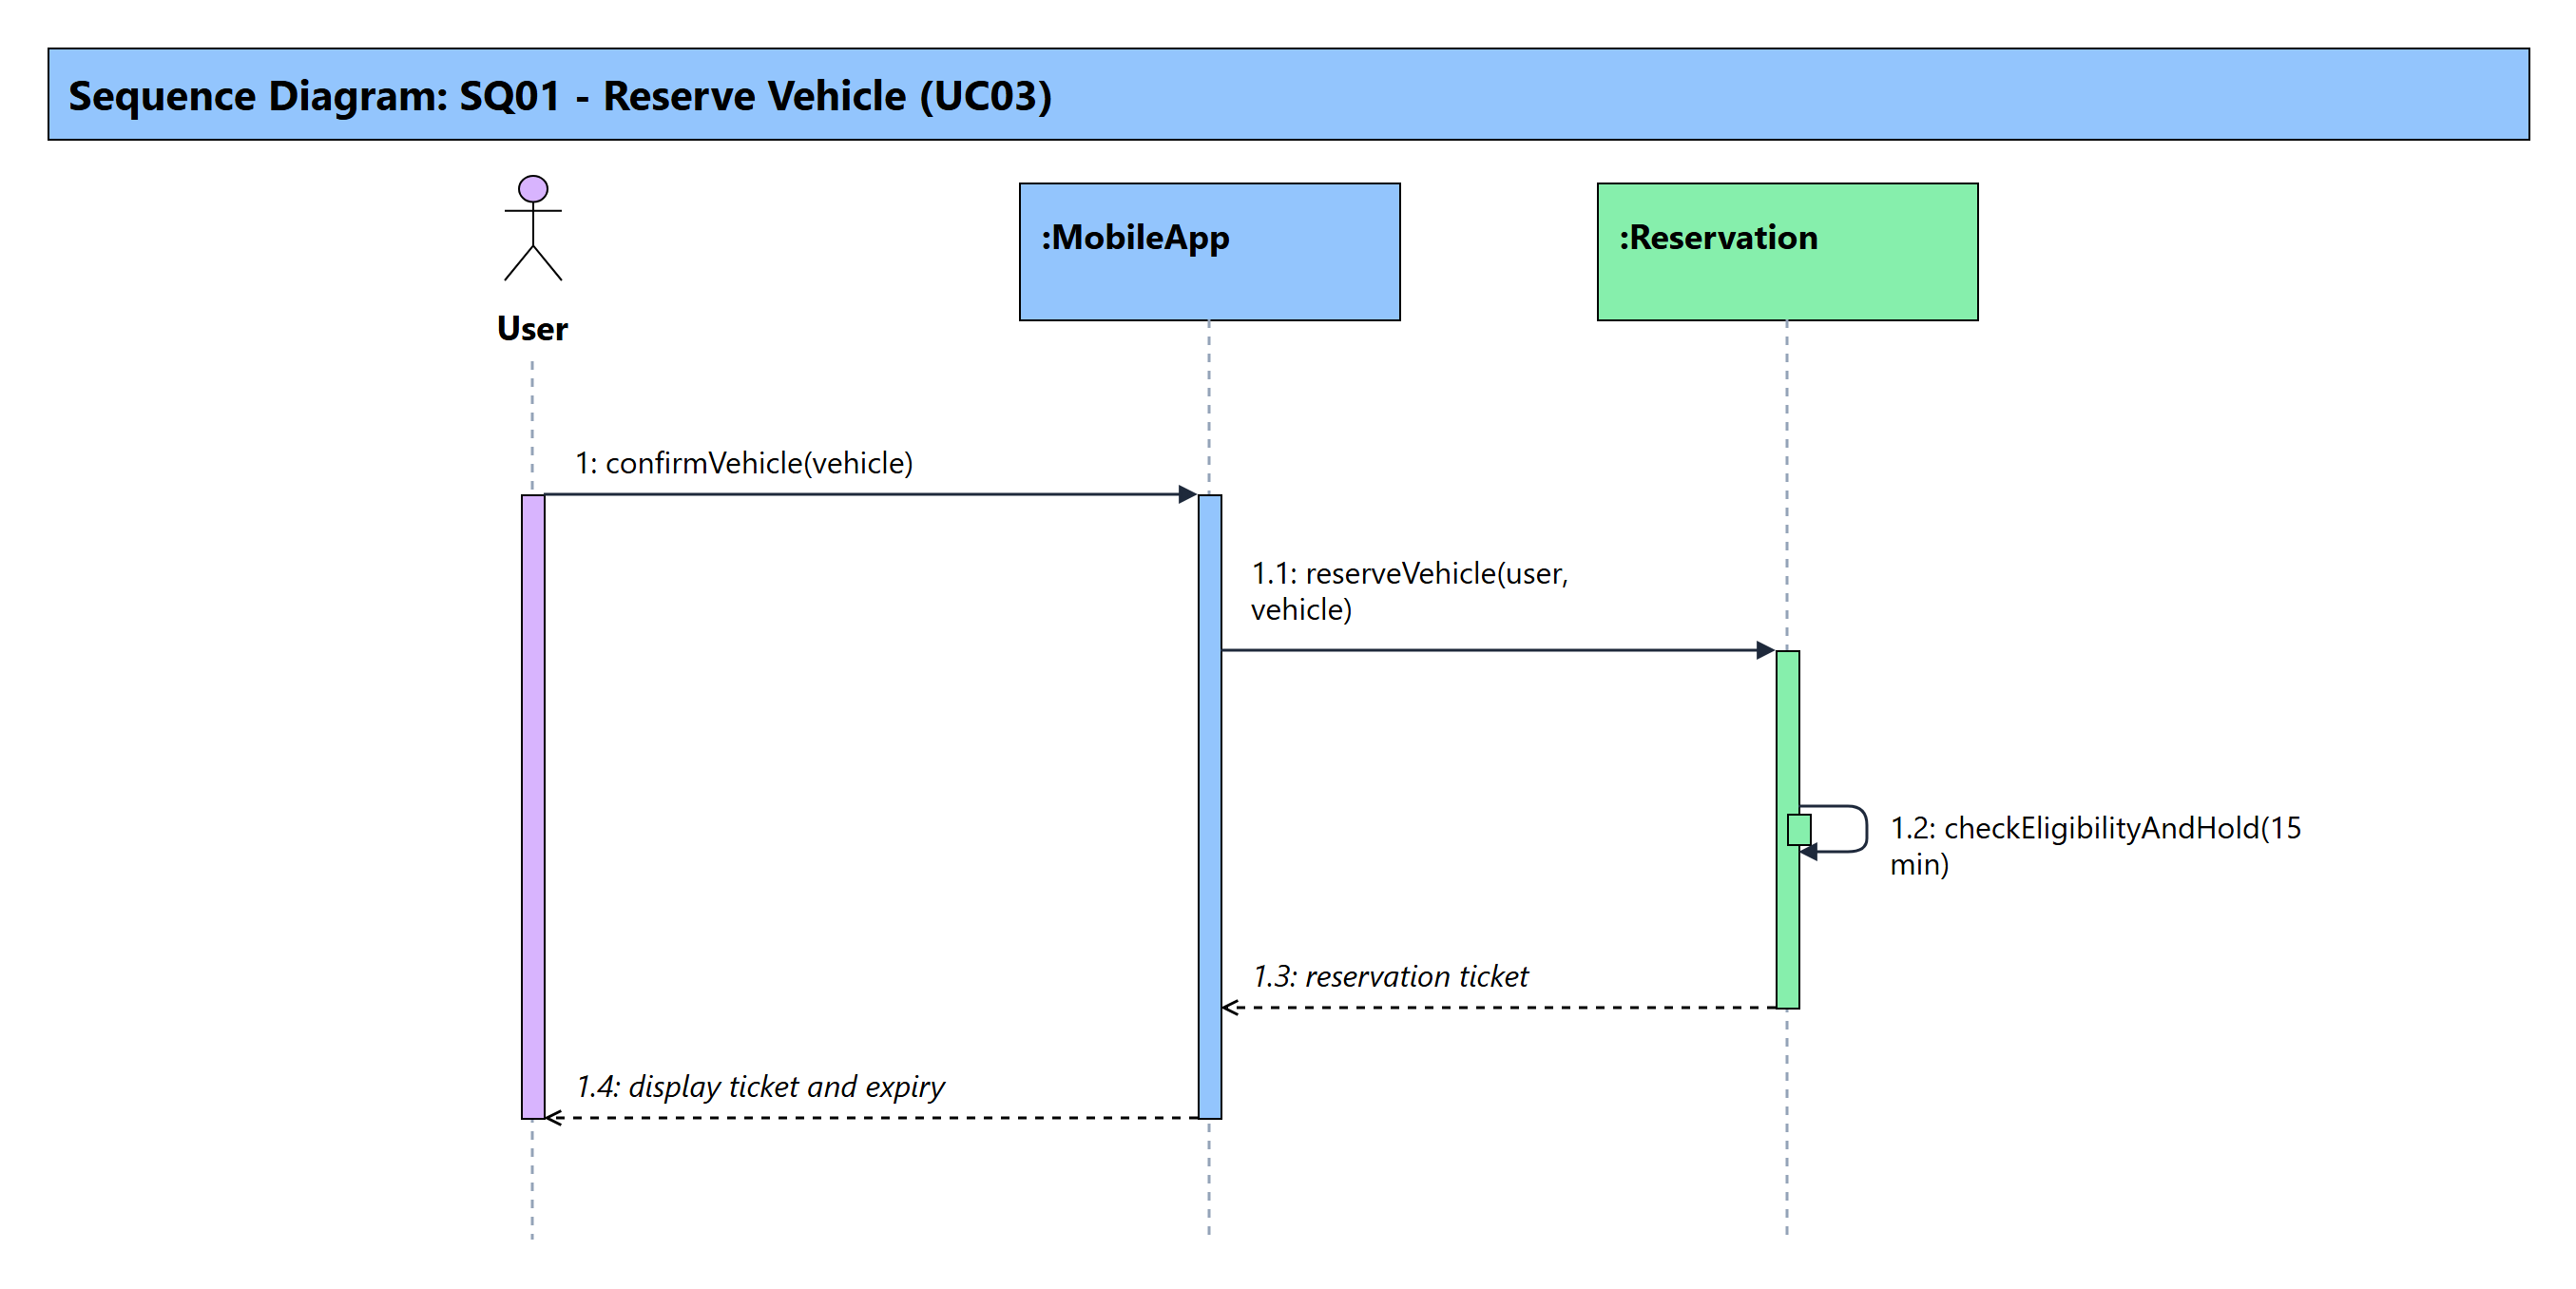
\includegraphics[width=0.92\textwidth,height=0.38\textheight,keepaspectratio]{graphics/diagrams/SQ01-Reserve_Vehicle.png}
    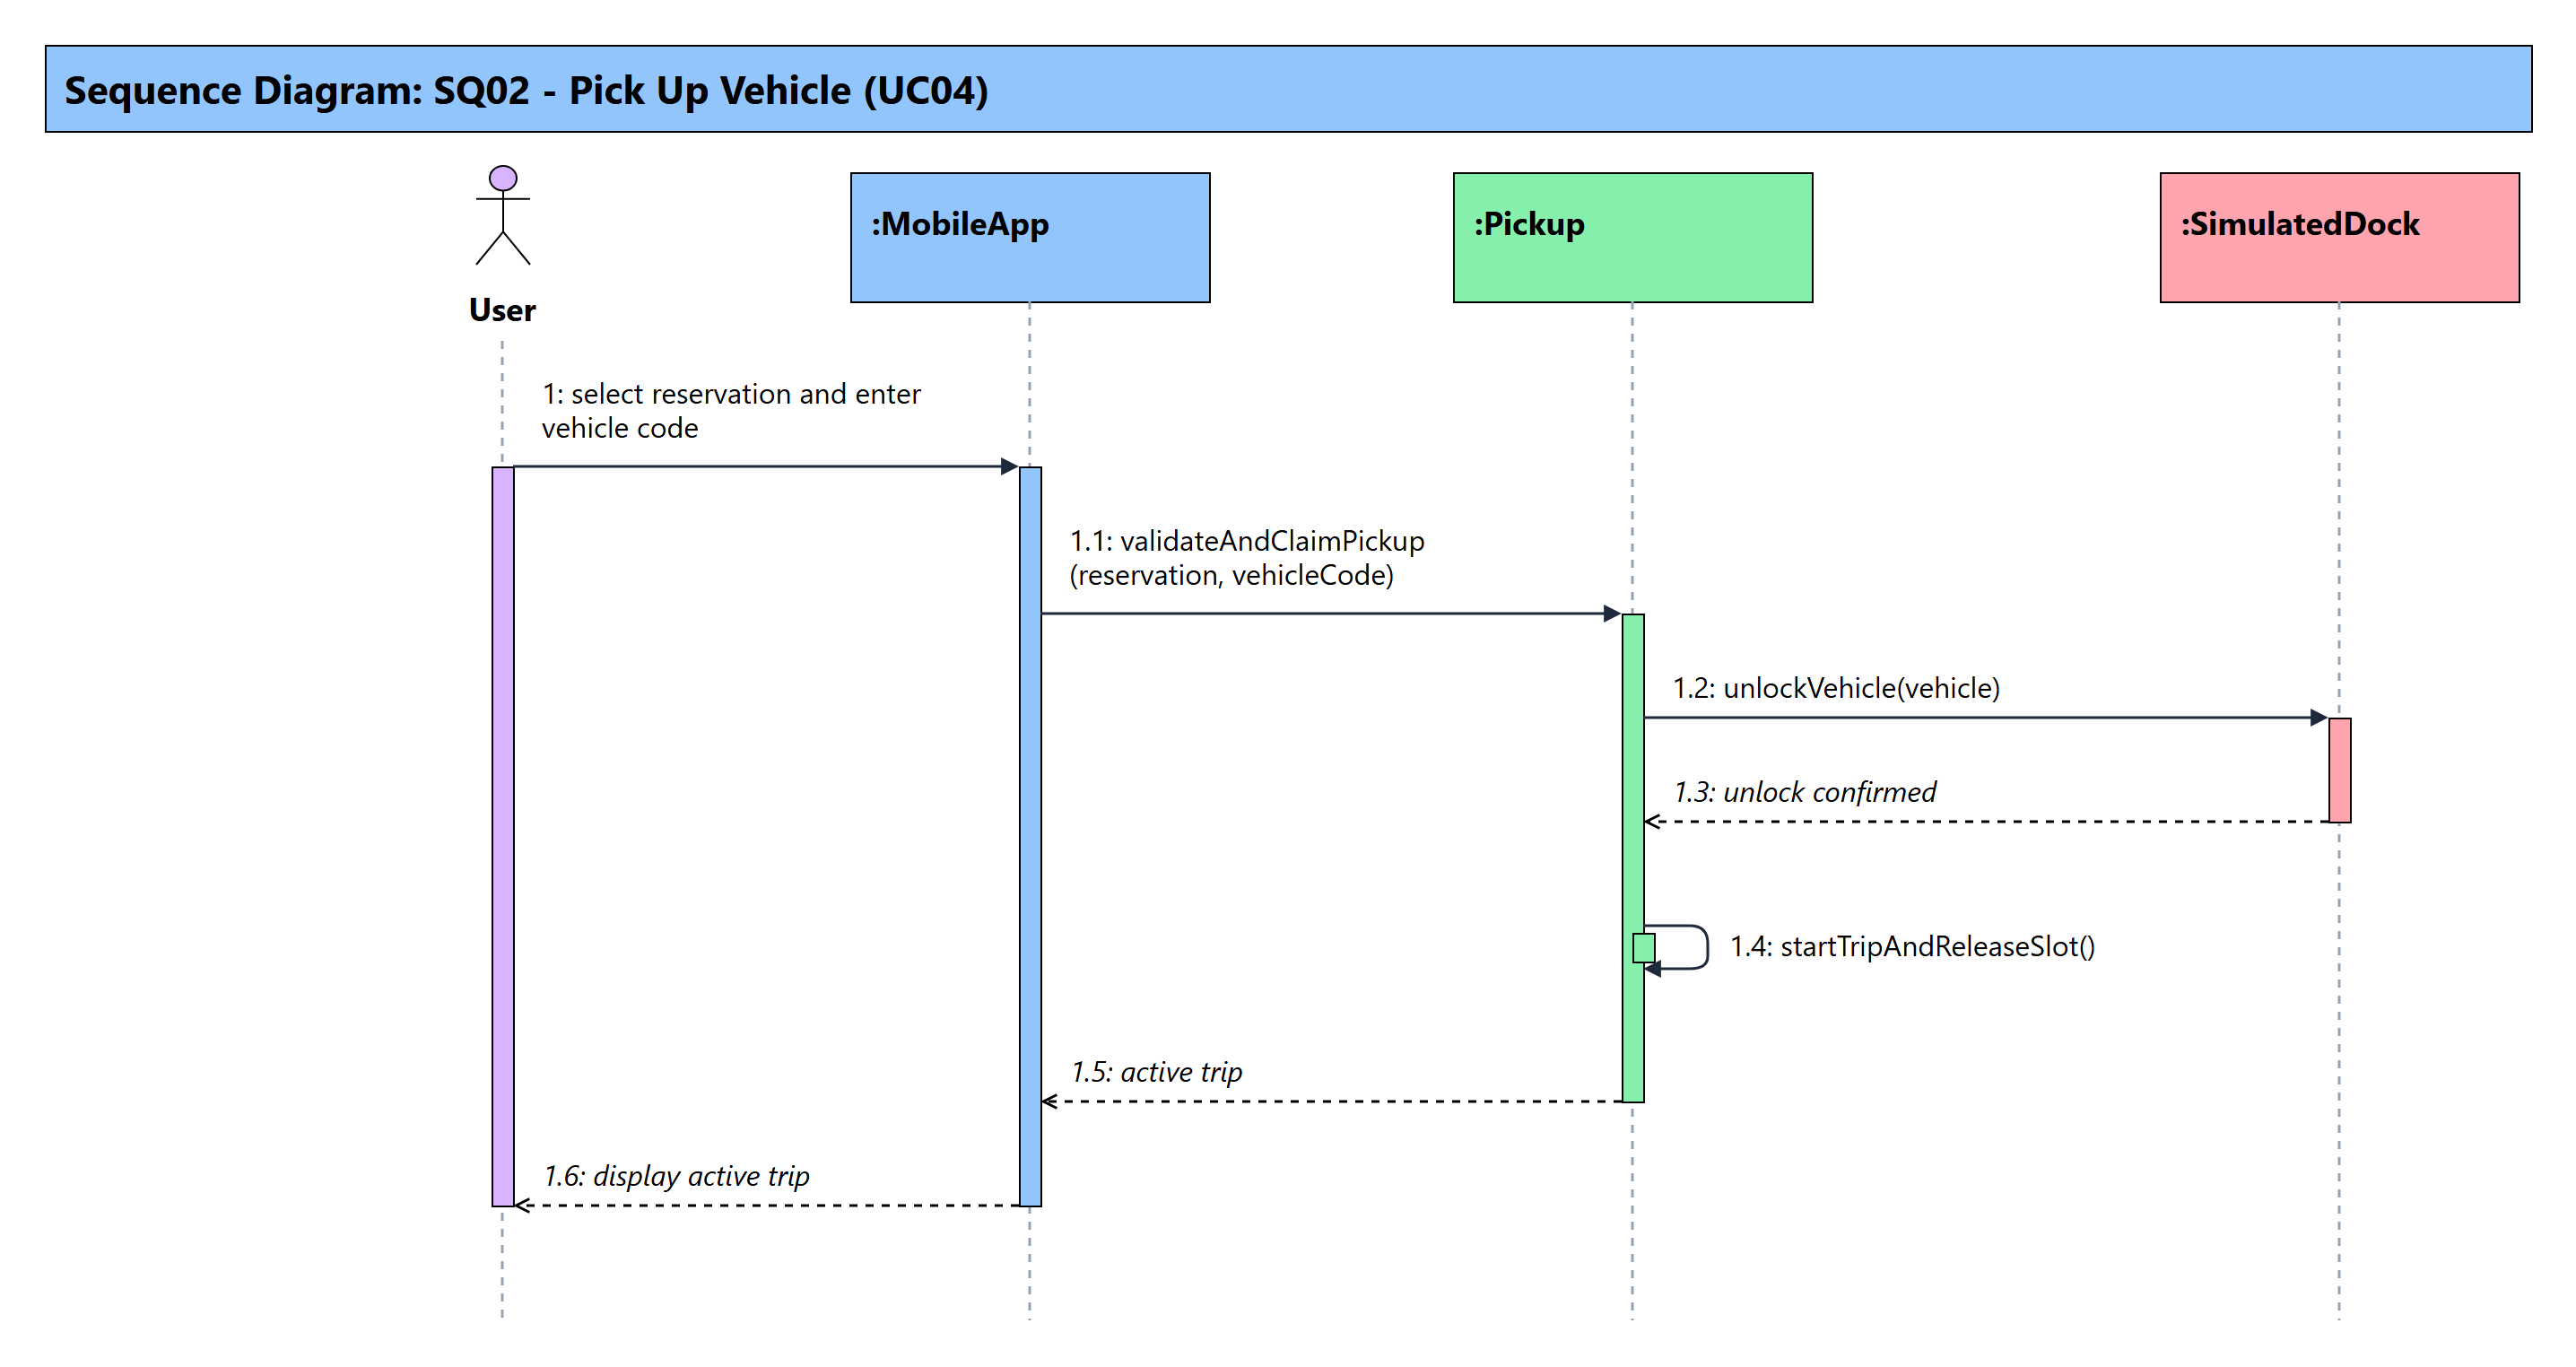
\includegraphics[width=0.92\textwidth,height=0.38\textheight,keepaspectratio]{graphics/diagrams/SQ02-Pick_Up_Vehicle.png}
    \caption{Sơ đồ tuần tự đặt giữ xe (\texttt{SQ01}) và nhận xe tại Hub (\texttt{SQ02})}
    \label{fig:sq-01-02}
\end{figure}

\begin{figure}[H]
    \centering
        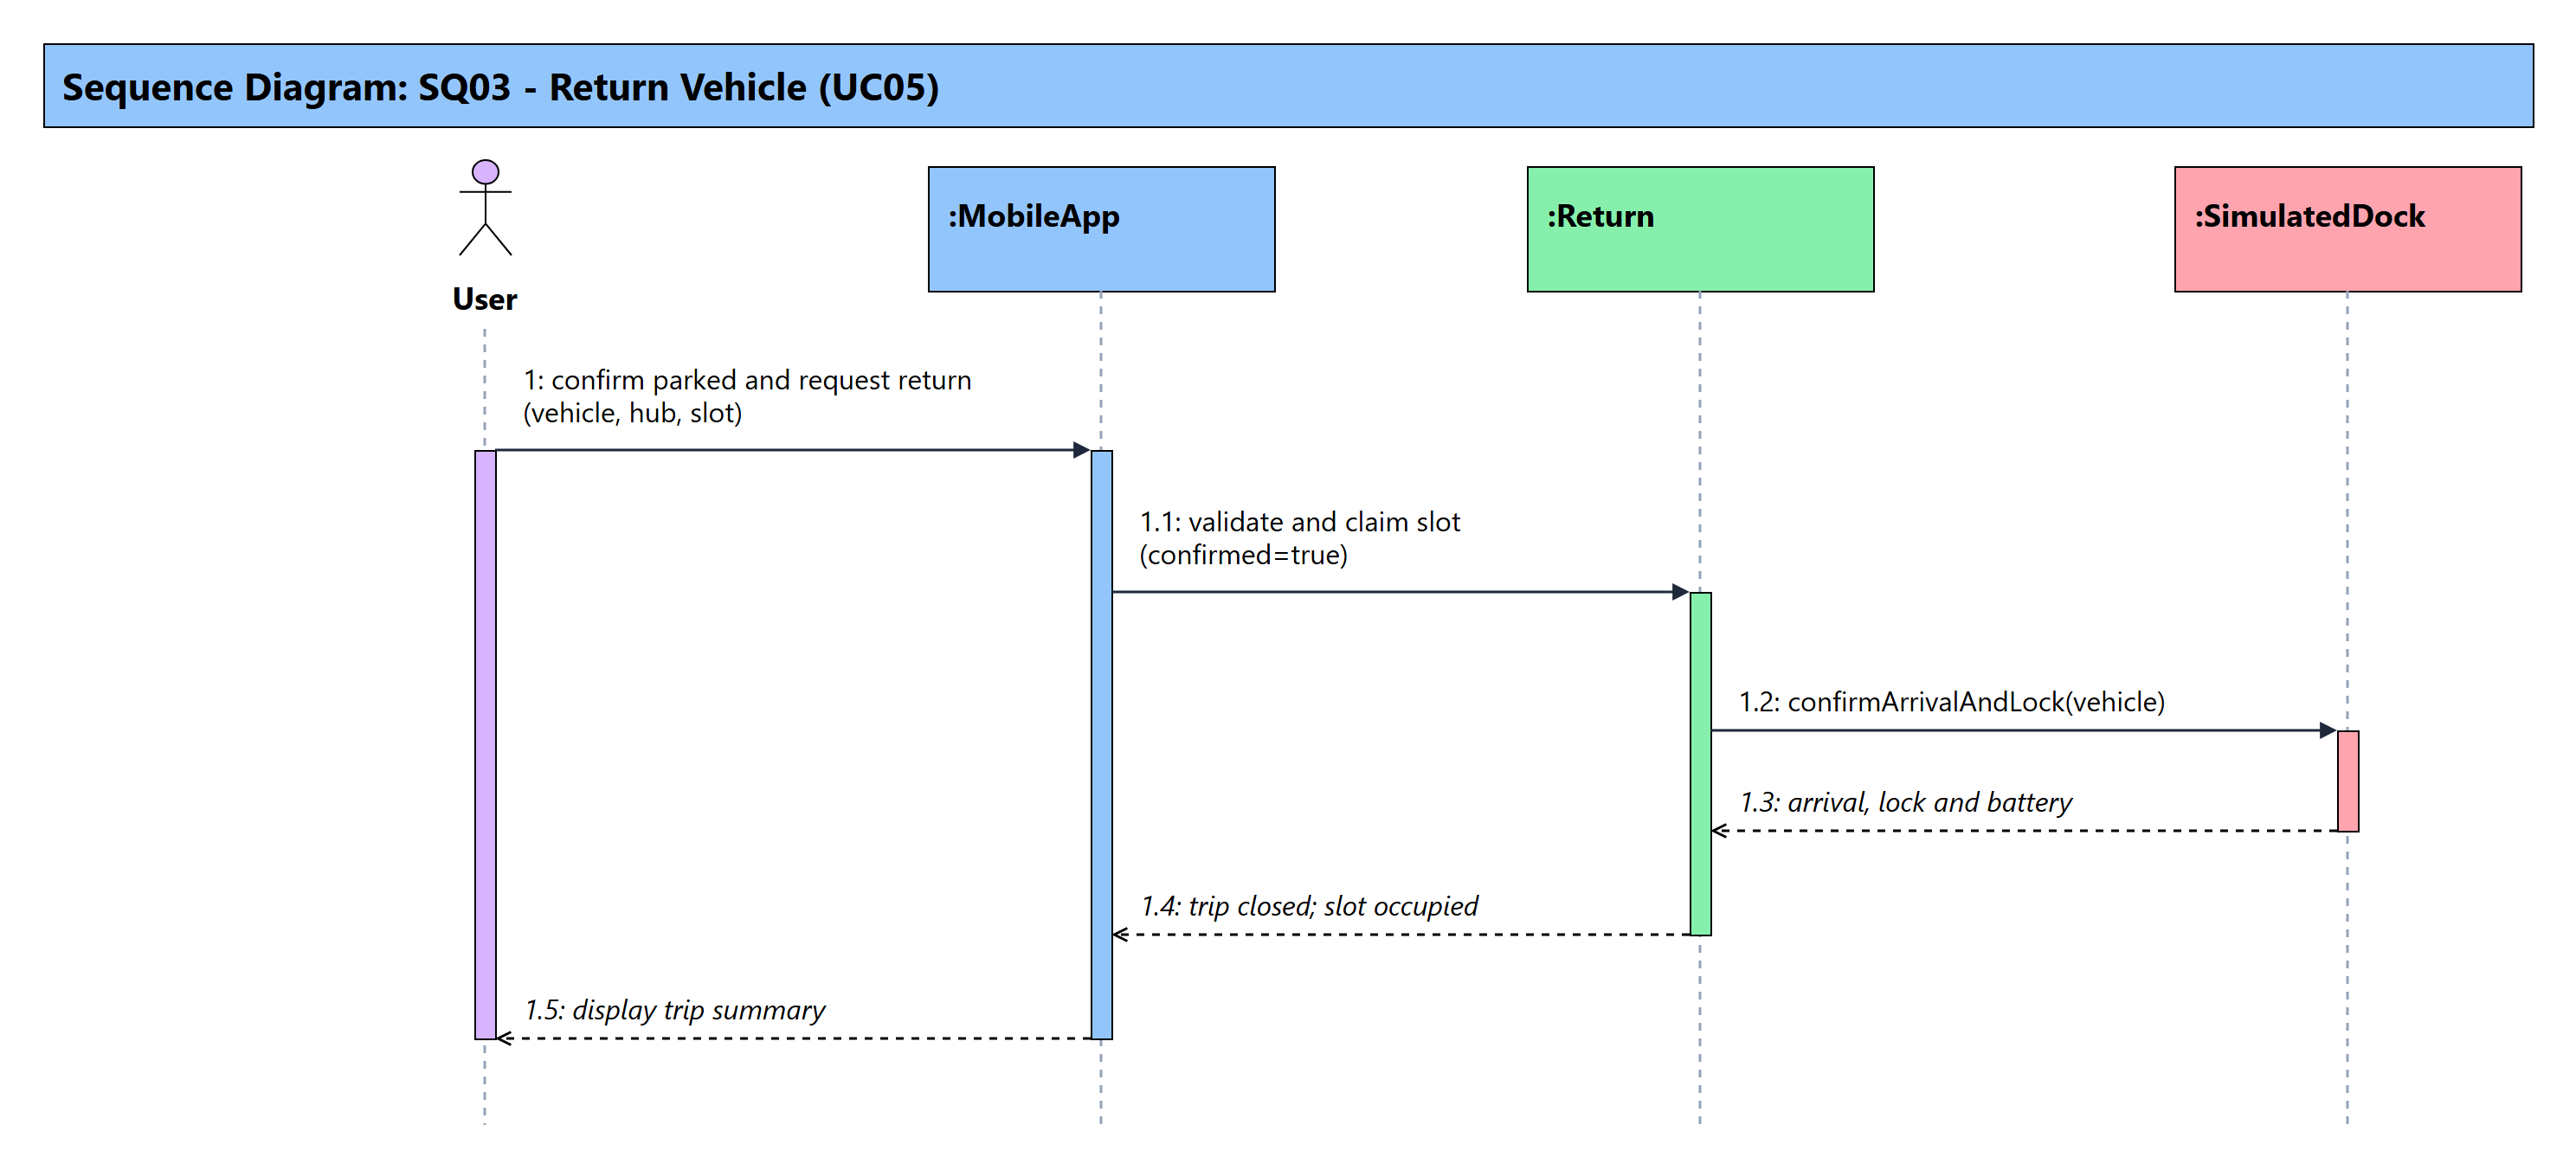
\includegraphics[width=0.92\textwidth,height=0.38\textheight,keepaspectratio]{graphics/diagrams/SQ03-Return_Vehicle.png}
    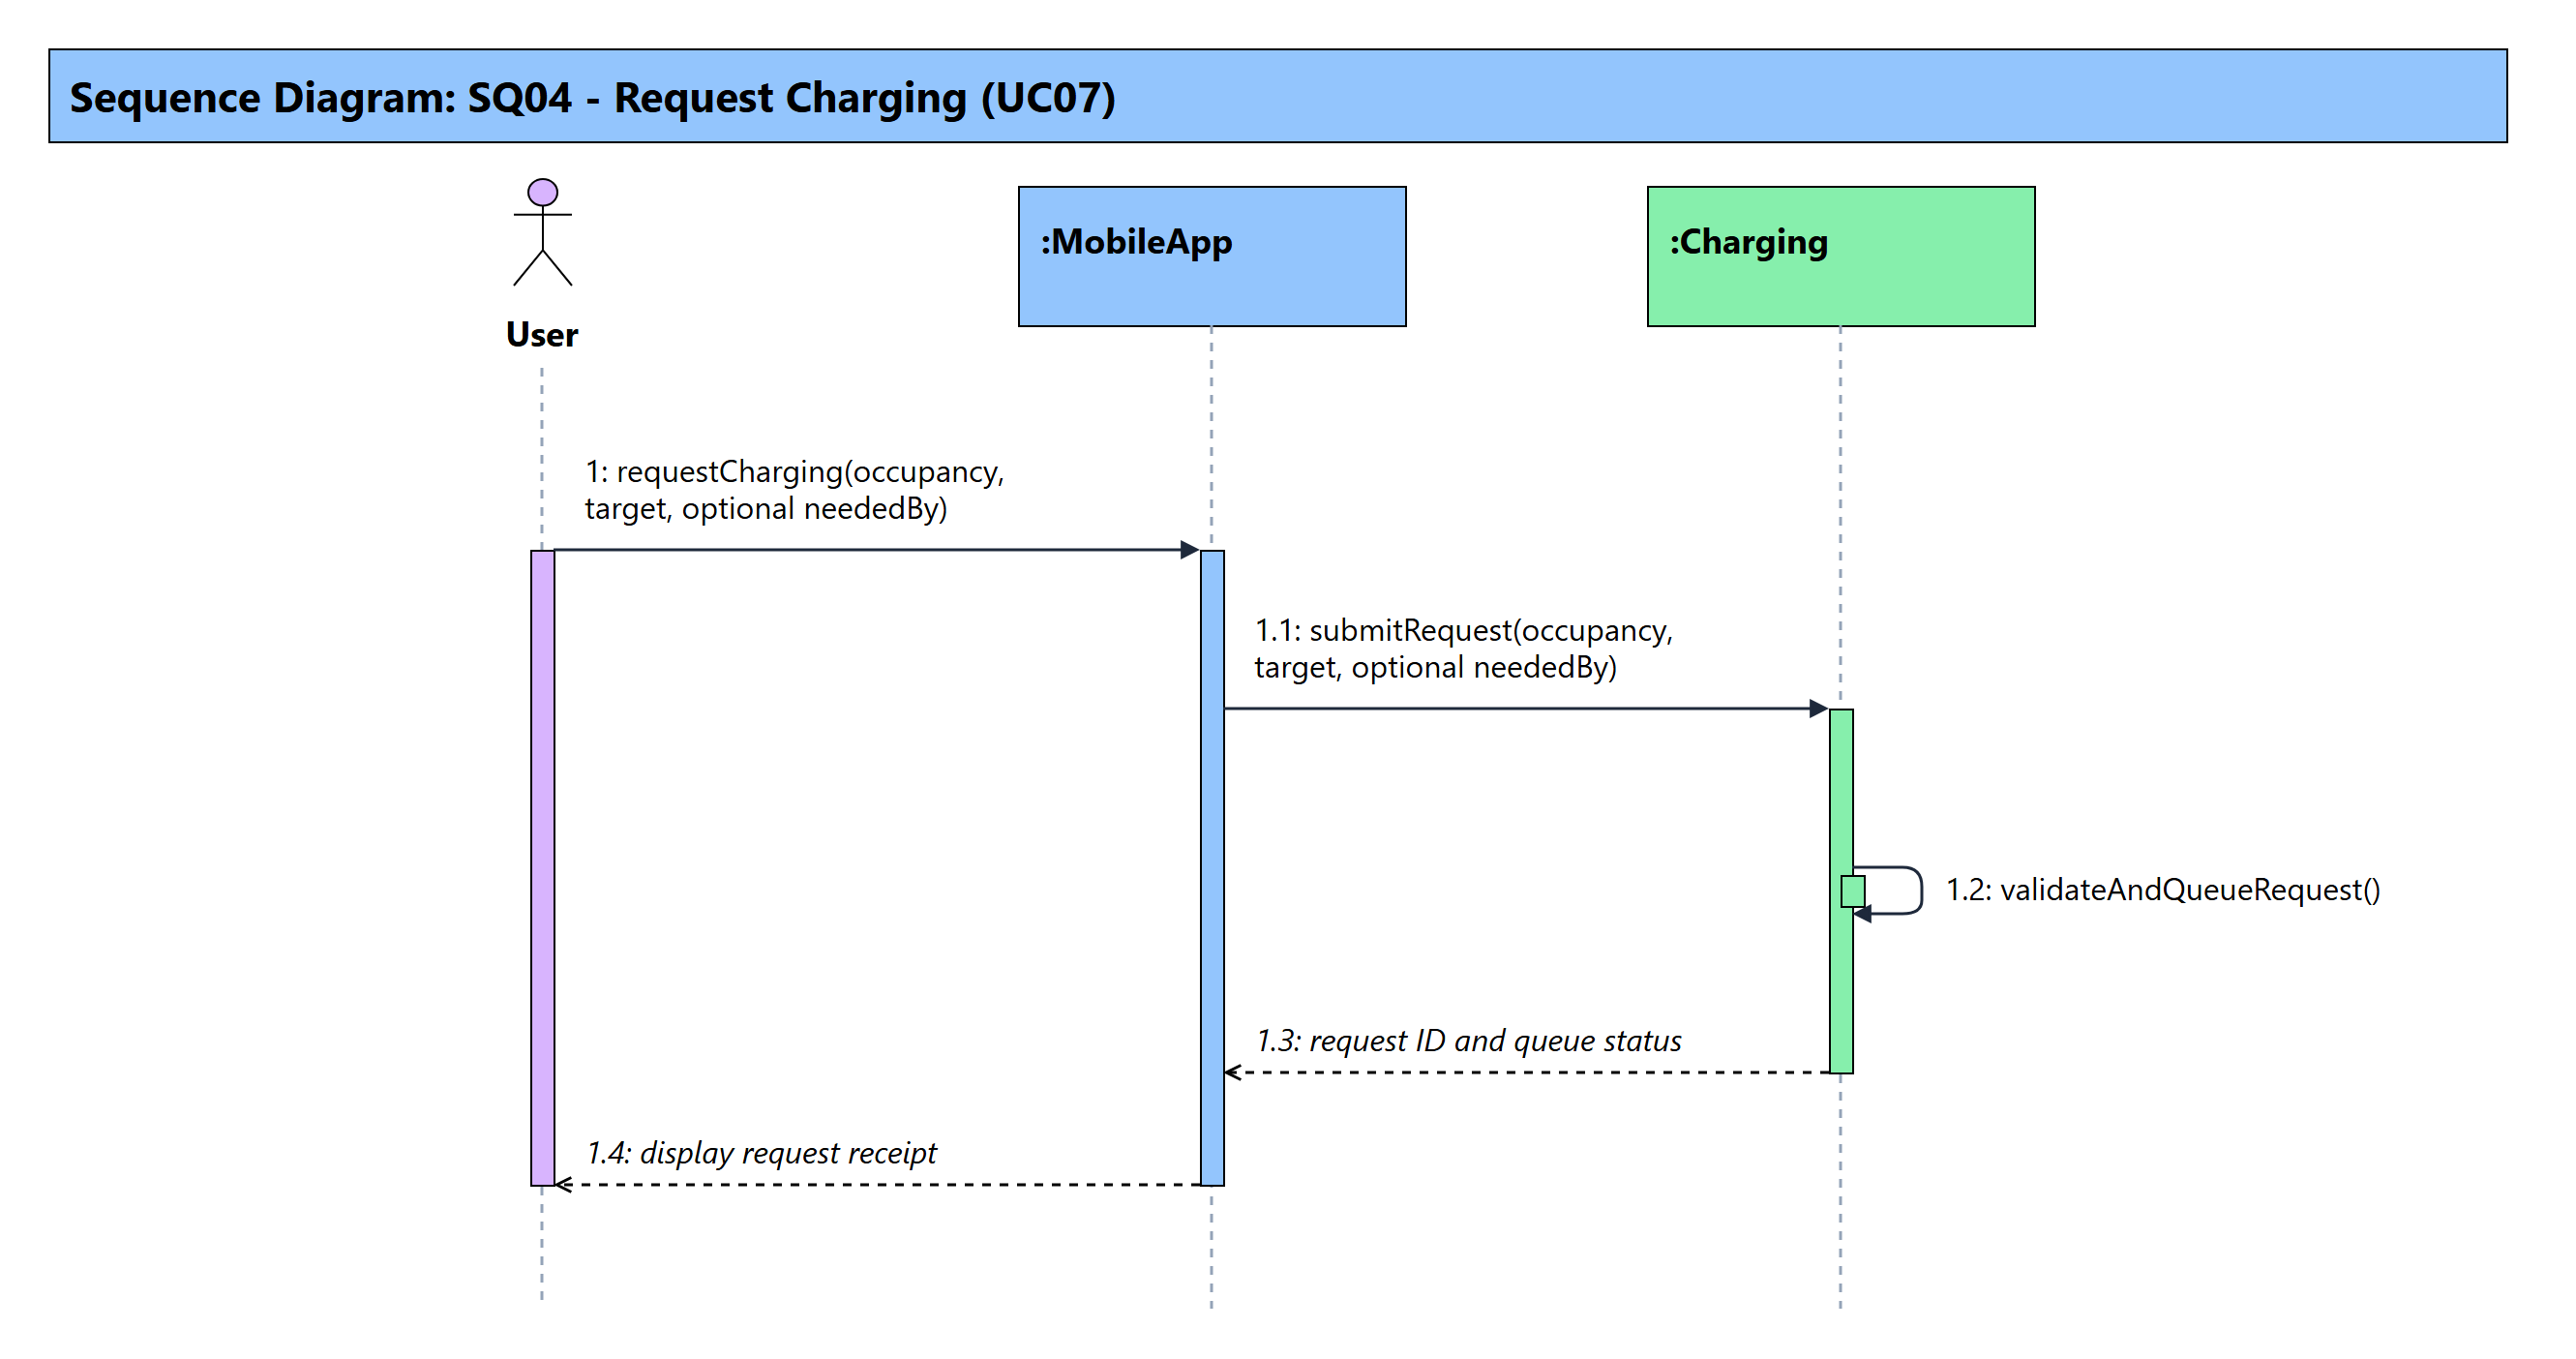
\includegraphics[width=0.92\textwidth,height=0.38\textheight,keepaspectratio]{graphics/diagrams/SQ04-Request_Charging.png}
    \caption{Sơ đồ tuần tự trả xe (\texttt{SQ03}) và tiếp nhận yêu cầu sạc (\texttt{SQ04})}
    \label{fig:sq-03-04}
\end{figure}

\begin{figure}[H]
    \centering
    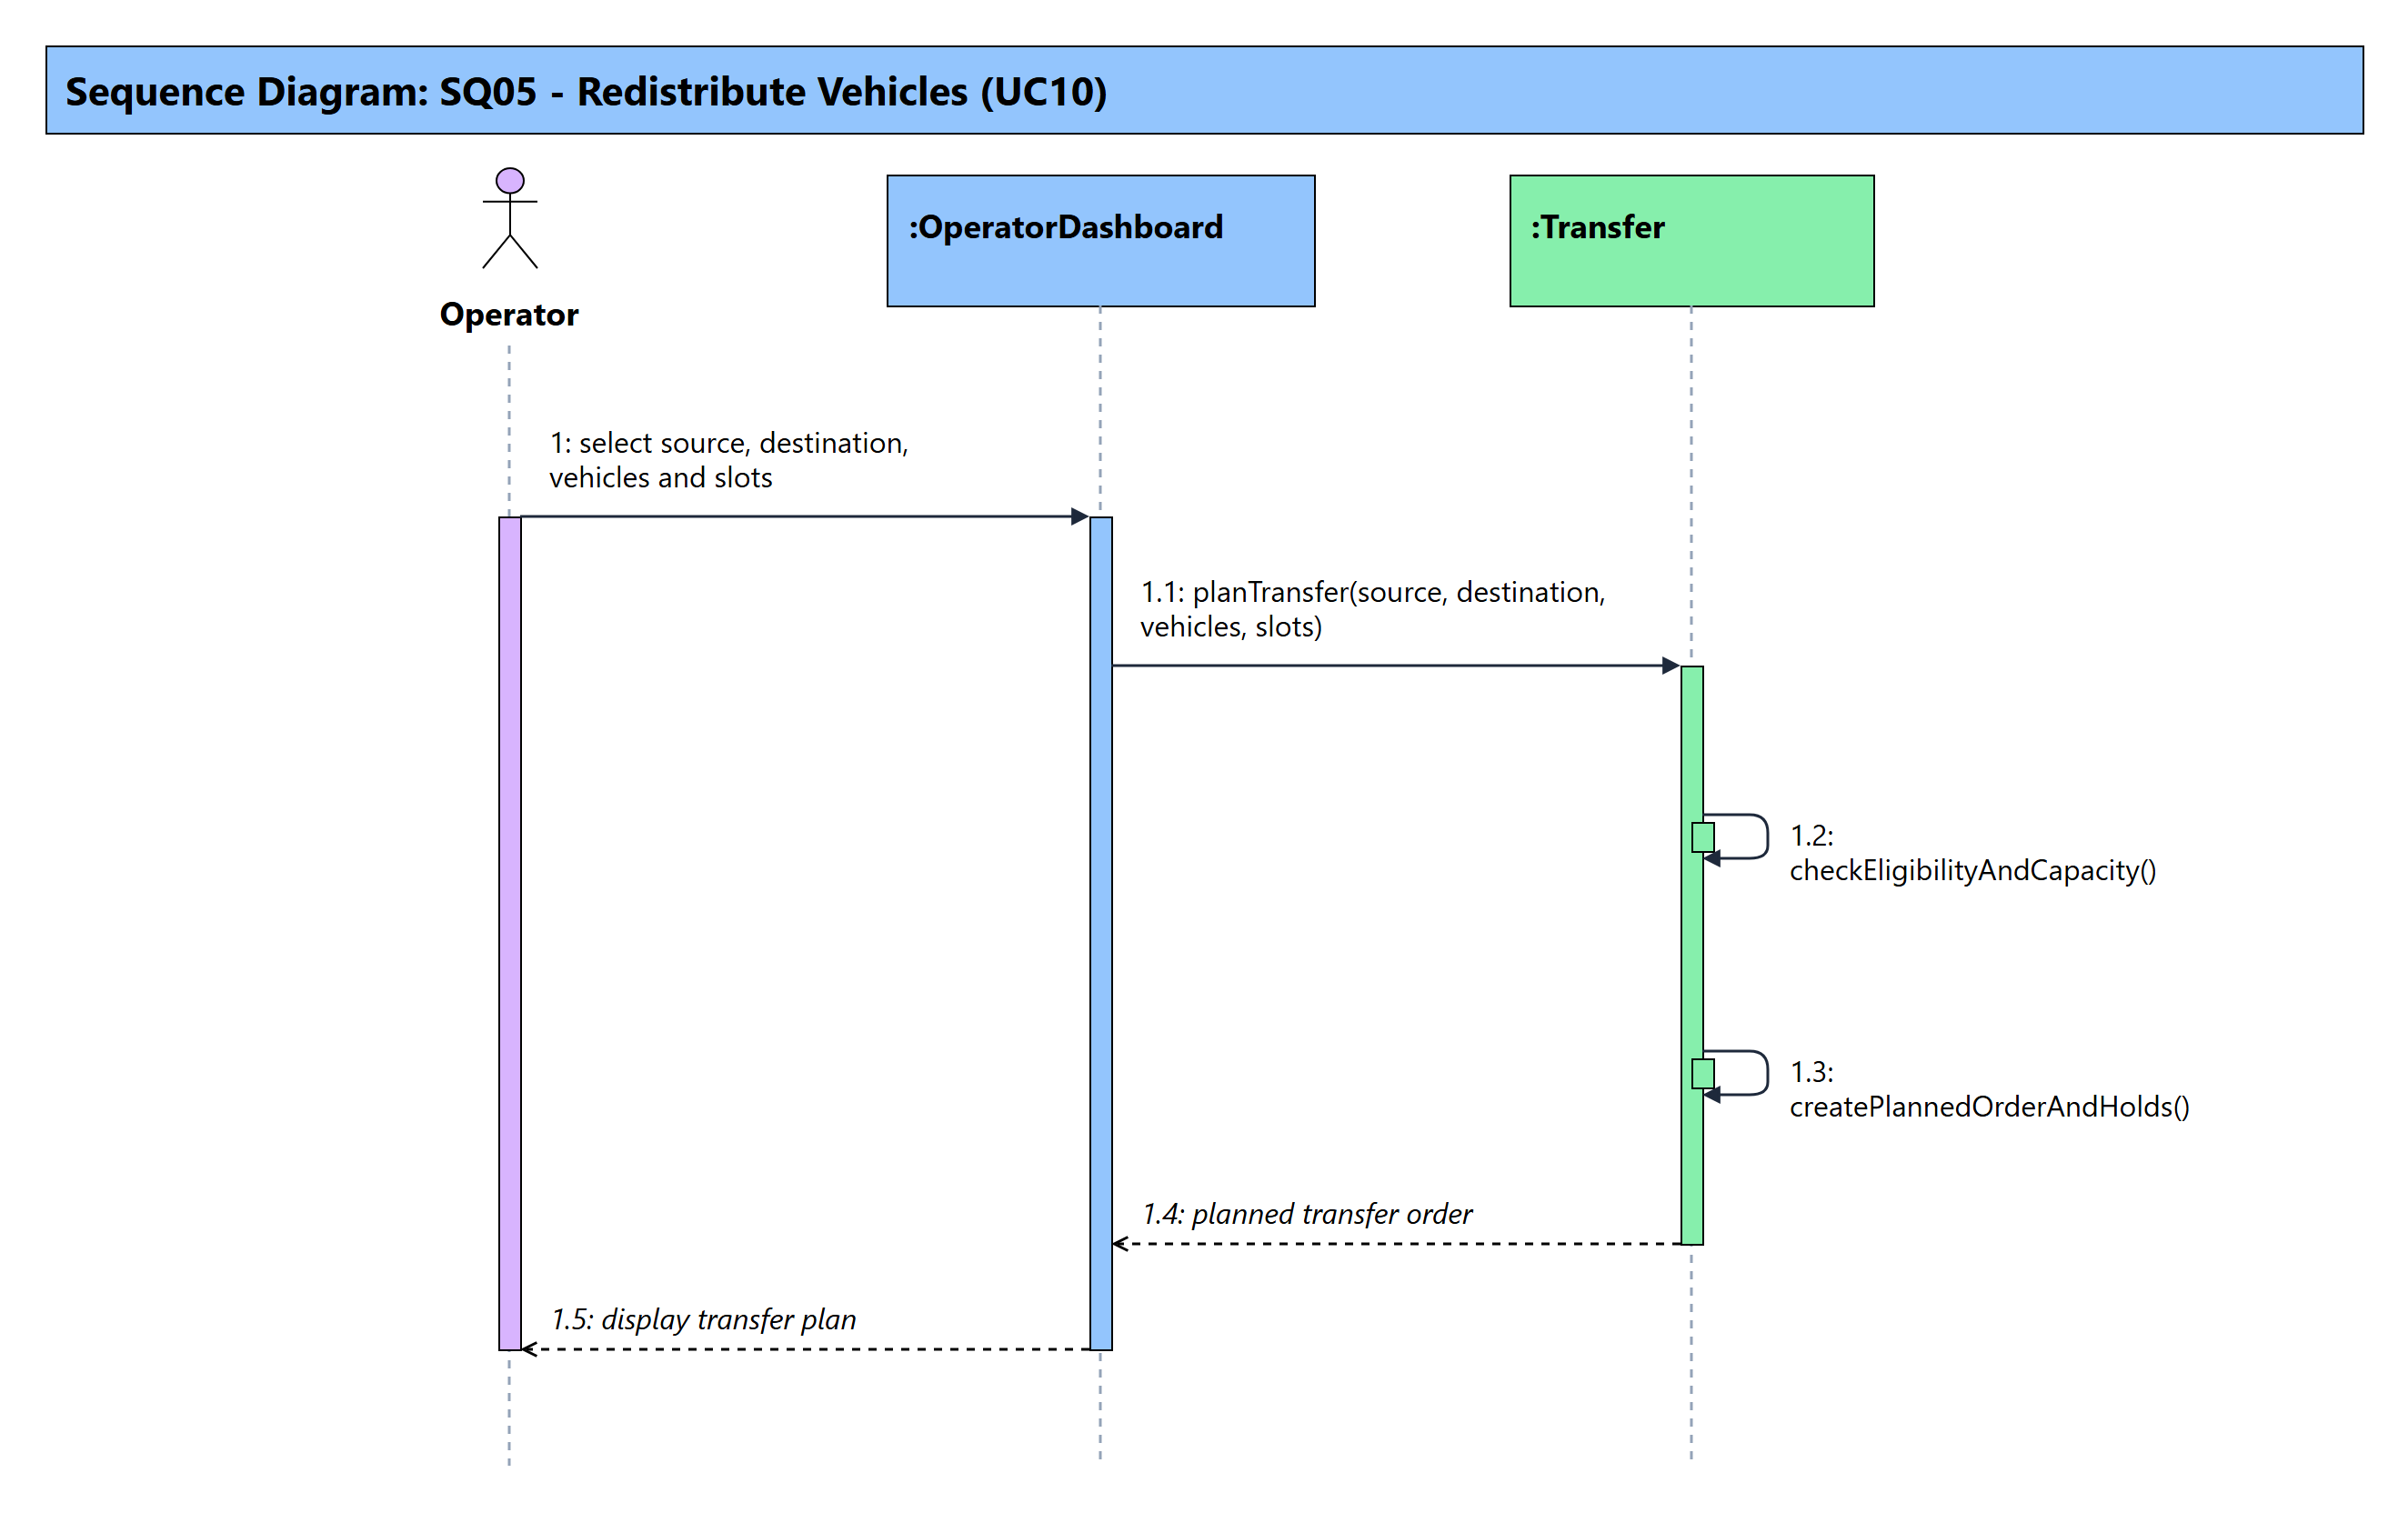
\includegraphics[width=0.92\textwidth,height=0.25\textheight,keepaspectratio]{graphics/diagrams/SQ05-Redistribute_Vehicles.png}\par\medskip
    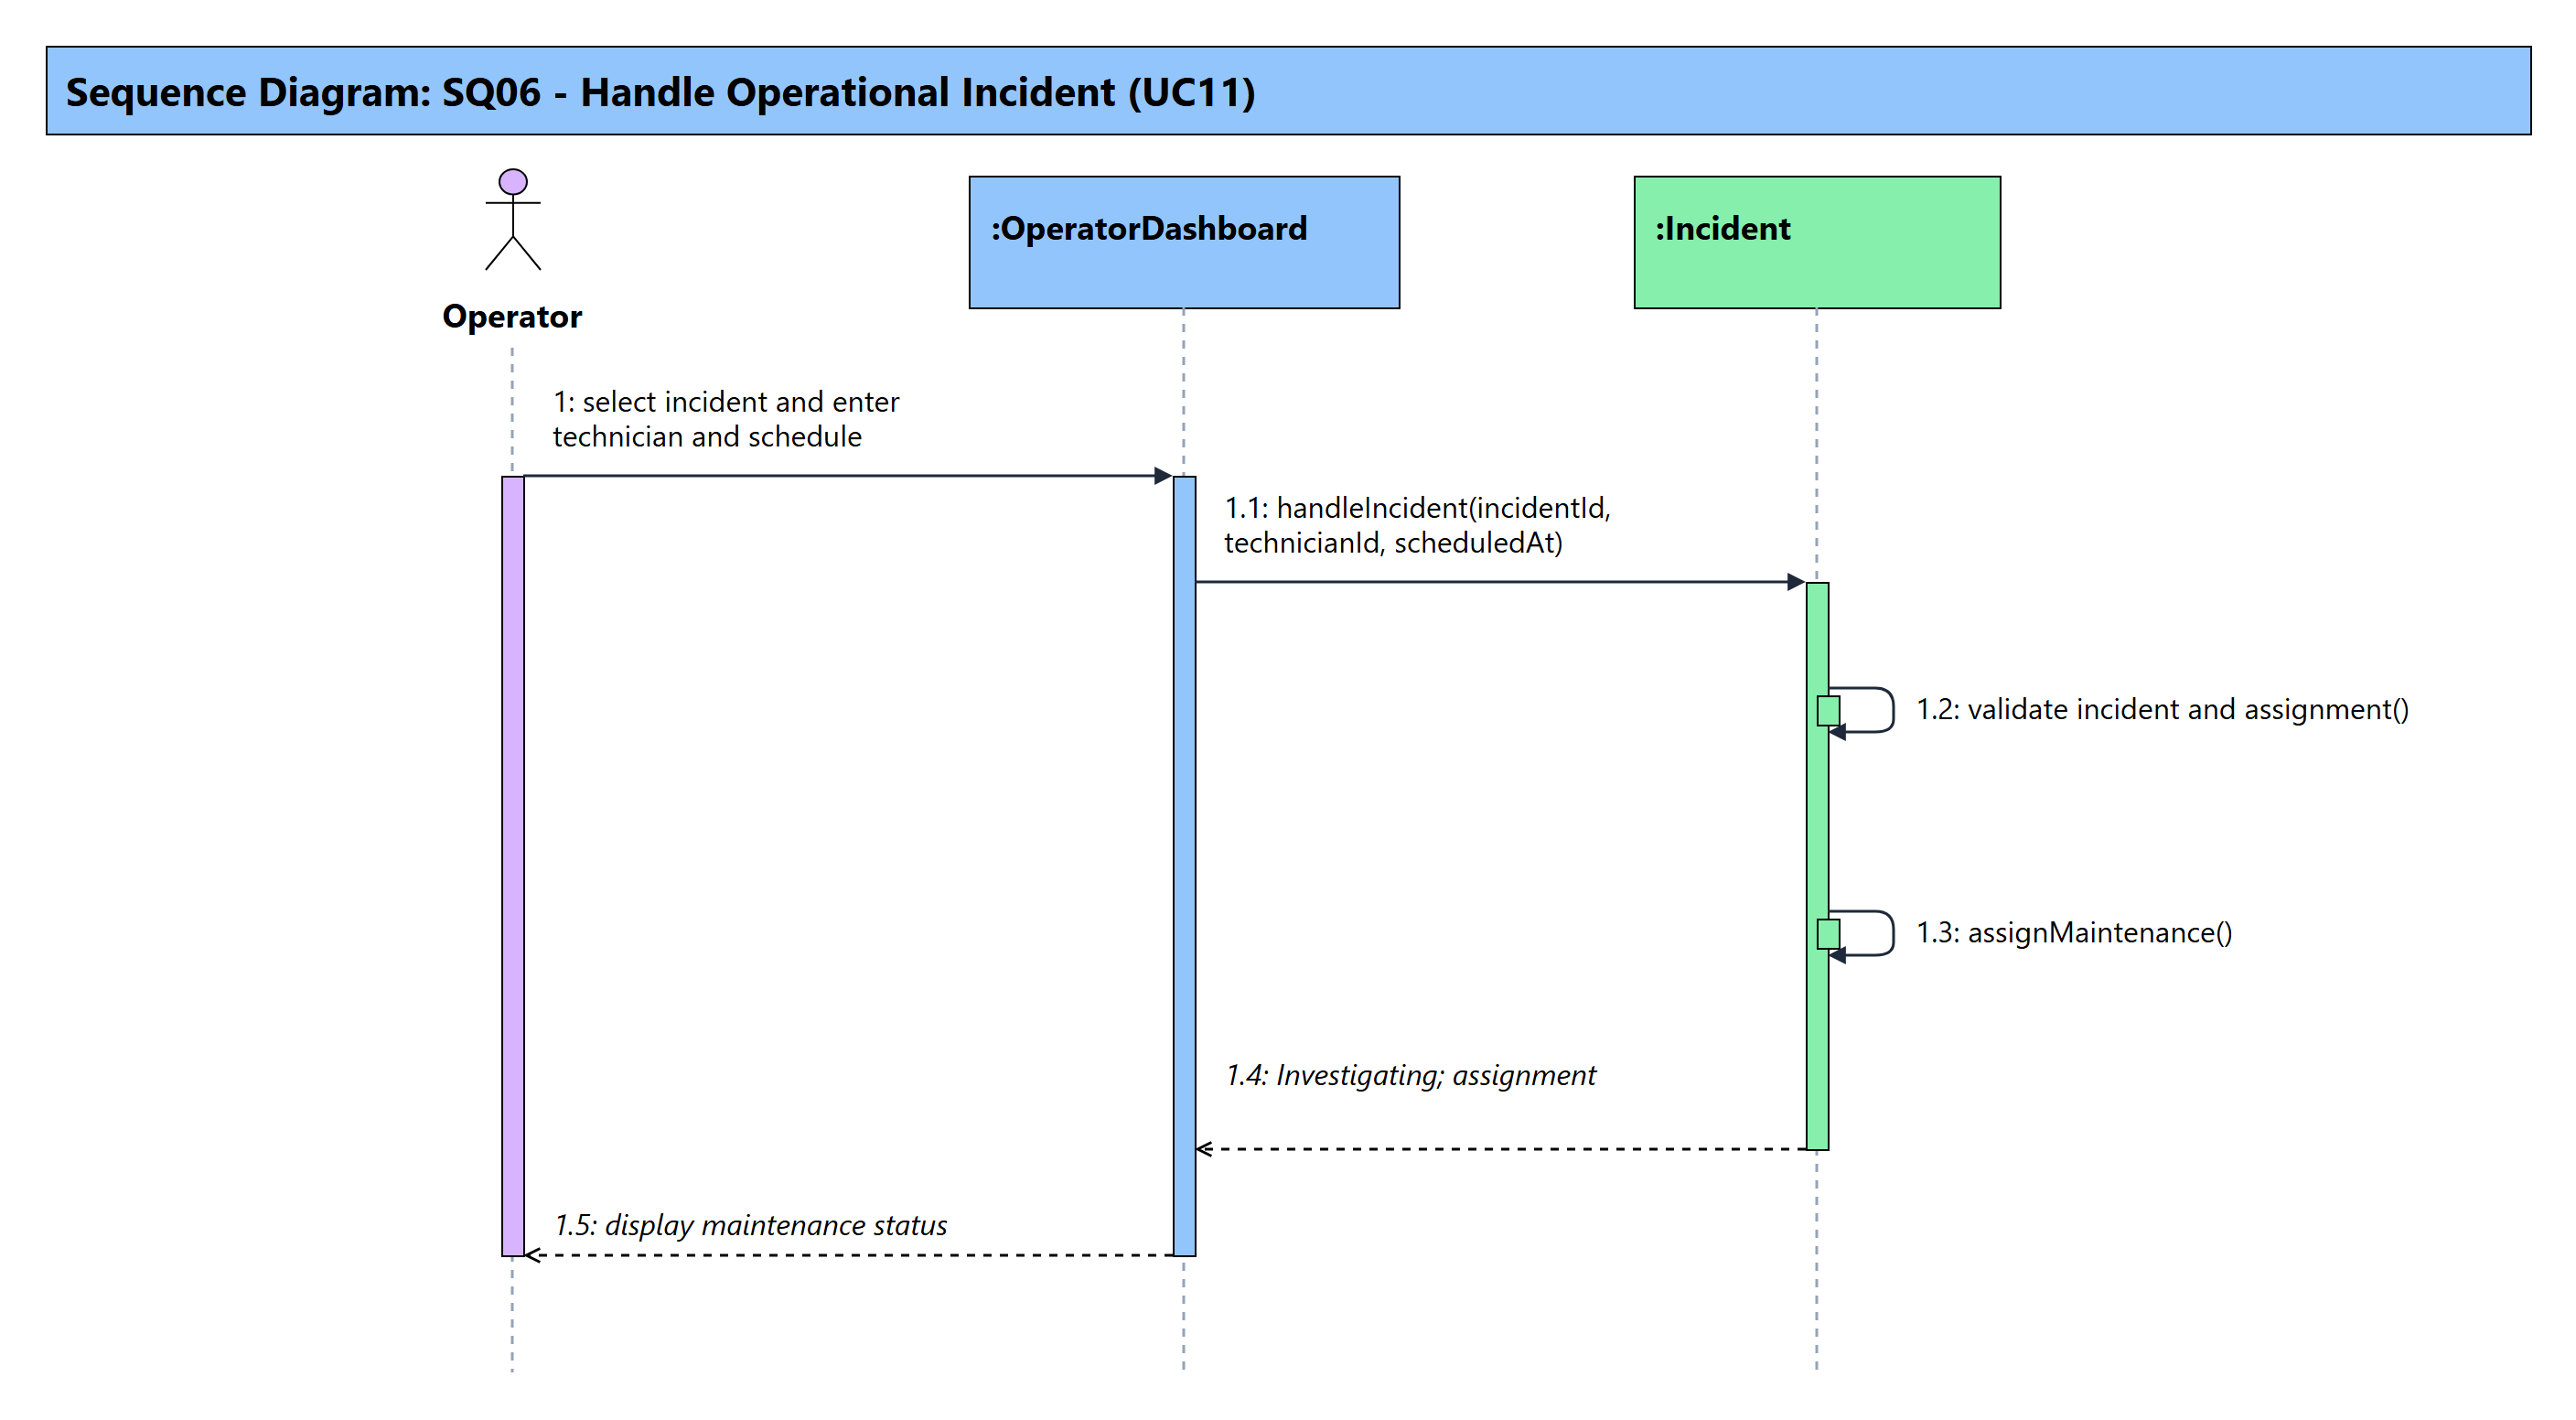
\includegraphics[width=0.92\textwidth,height=0.25\textheight,keepaspectratio]{graphics/diagrams/SQ06-Handle_Operational_Incident.png}\par\medskip
    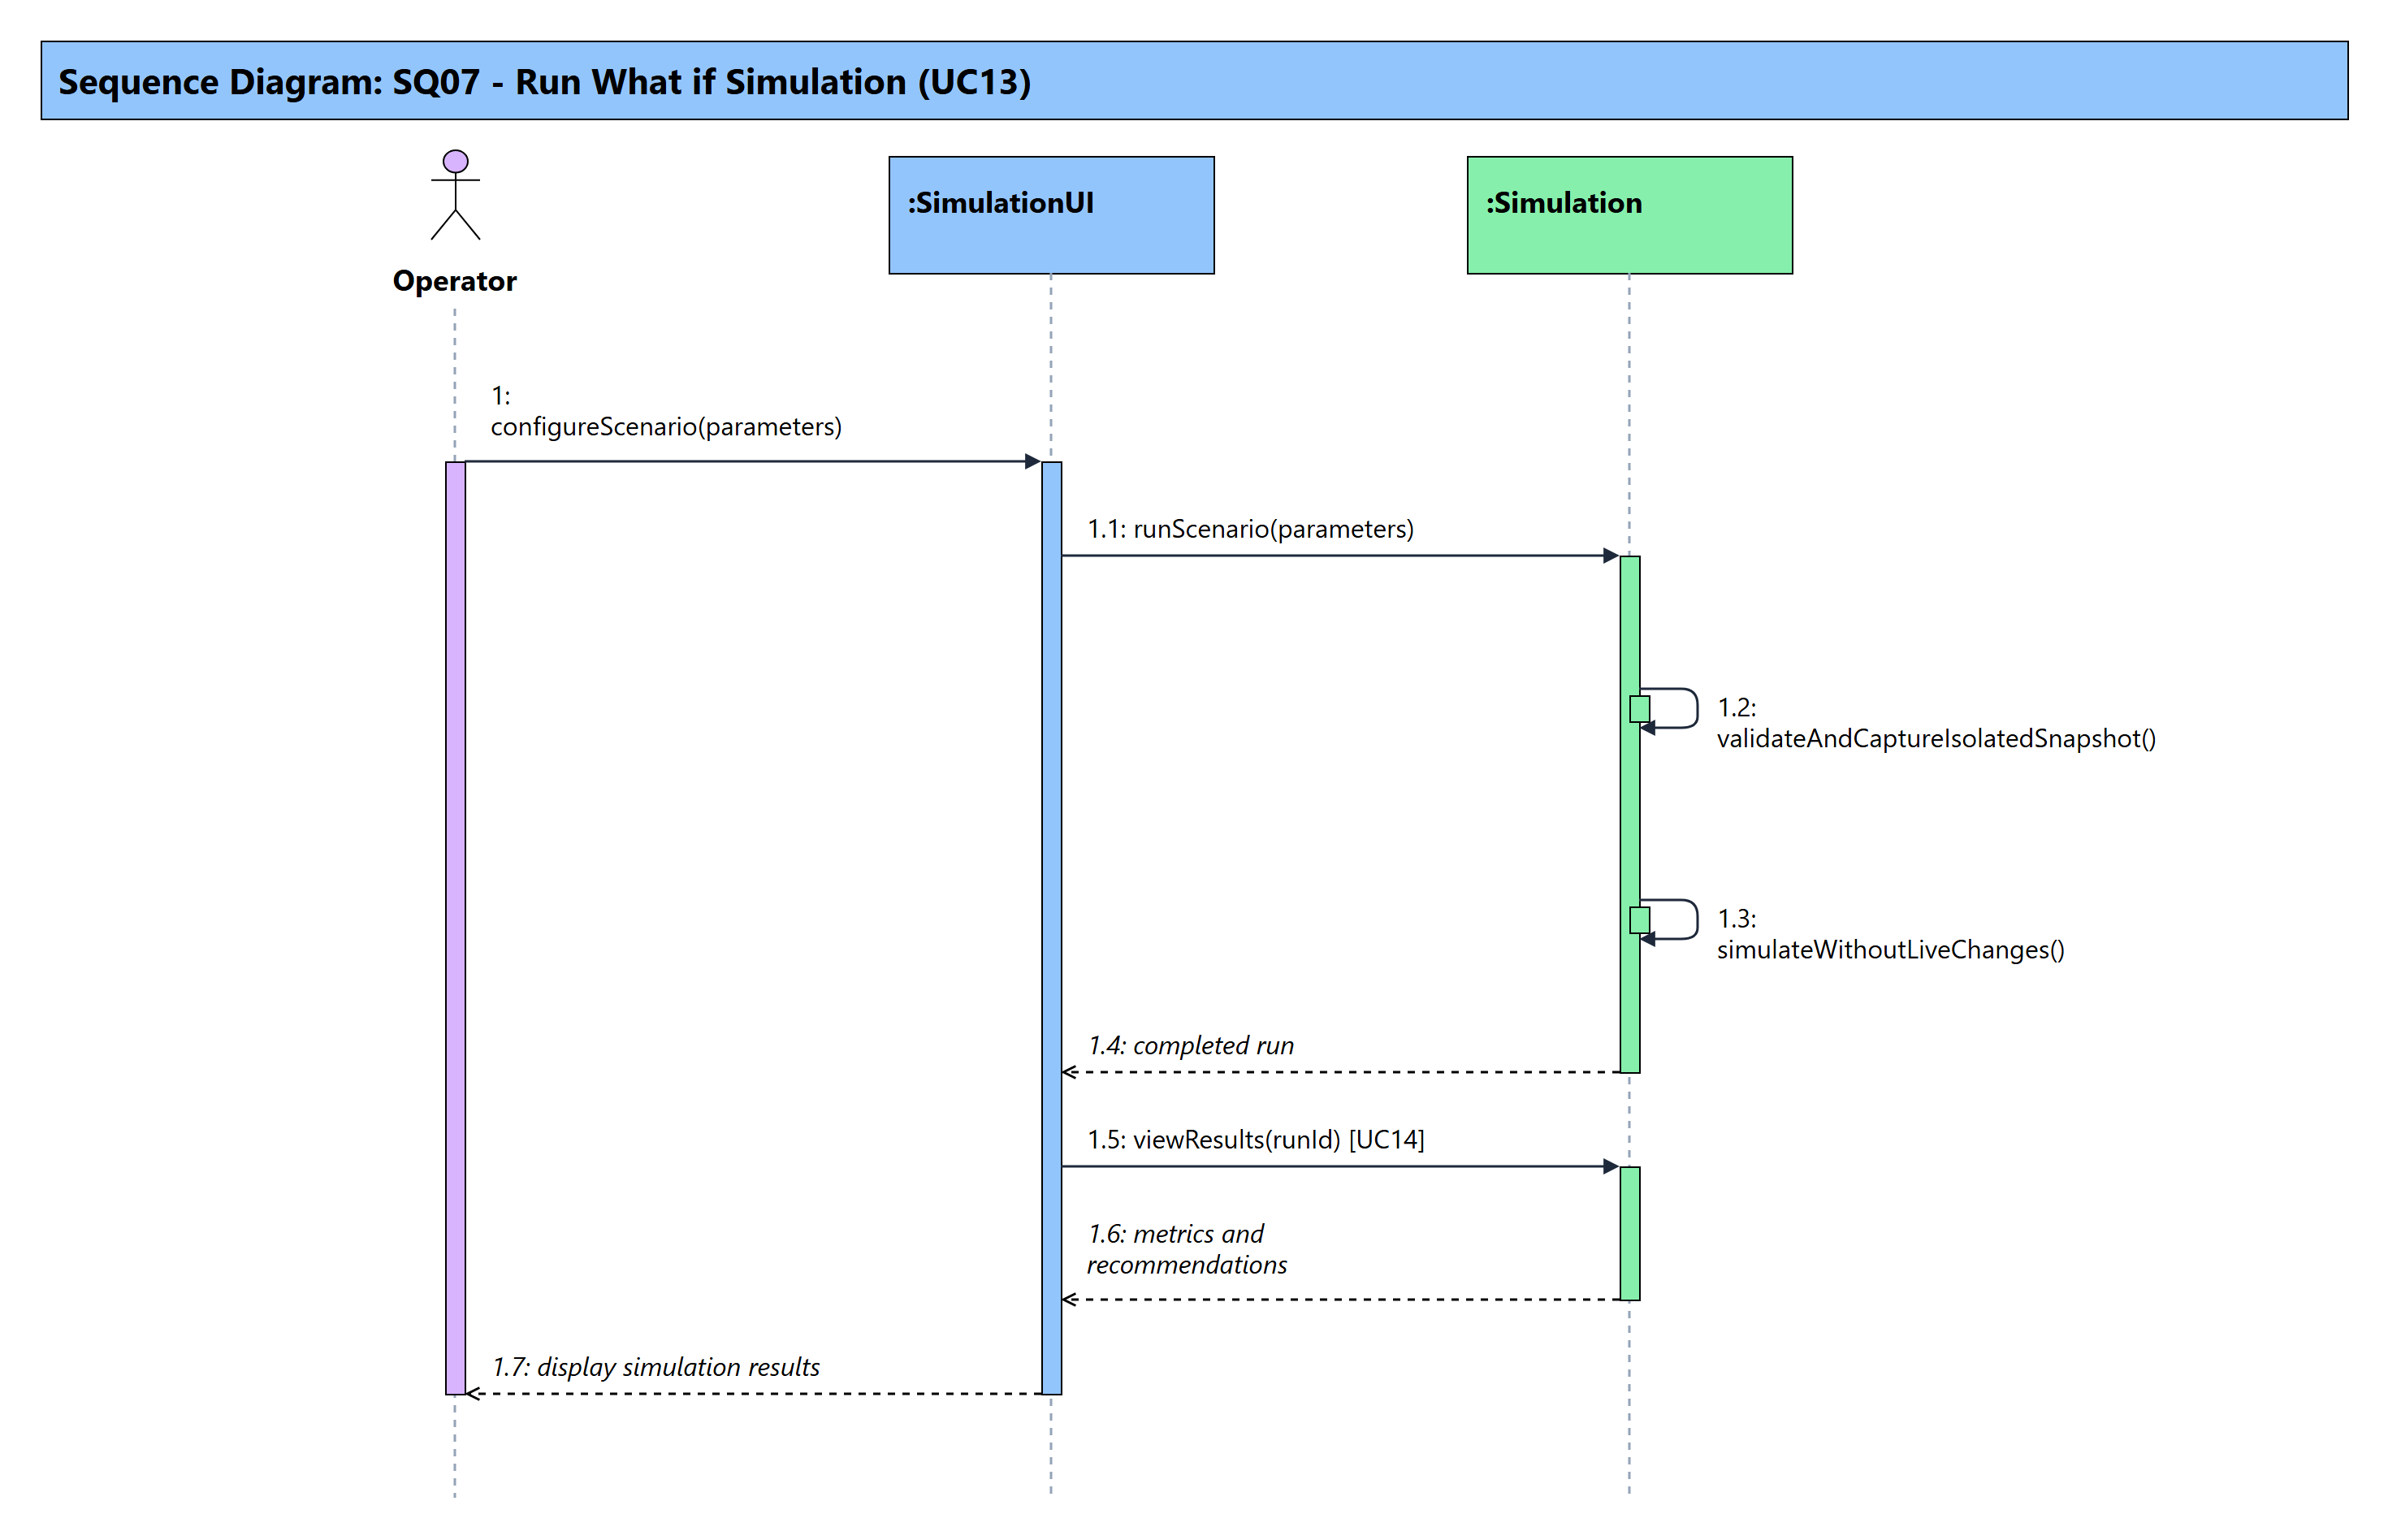
\includegraphics[width=0.92\textwidth,height=0.25\textheight,keepaspectratio]{graphics/diagrams/SQ07-Run_What_if_Simulation.png}
    \caption{Sơ đồ tuần tự điều chuyển xe (\texttt{SQ05}), xử lý sự cố (\texttt{SQ06}) và mô phỏng What-if (\texttt{SQ07})}
    \label{fig:sq-05-07}
\end{figure}

\subsection{Mô hình Hành vi: Sơ đồ Hoạt động (Activity Diagrams -- AD01--AD07)}

Bộ 7 sơ đồ hoạt động được tổ chức theo các đường bơi (\textit{Swimlanes}) phân định trách nhiệm giữa \texttt{User / App} (hoặc \texttt{Operator / App}), \texttt{Backend} và \texttt{IoT / Simulated Station}. Mọi nút rẽ nhánh đều gắn điều kiện bảo vệ (\textit{guard condition}) như \texttt{[Available, battery >=20\%, no hold]}, bảo đảm mọi nhánh xung đột hoặc ngoại lệ đều dẫn về nút kết thúc hợp lệ (\Cref{tab:ad-overview} và \Cref{fig:ad-01}--\Cref{fig:ad-07}). Đặc biệt, \texttt{AD04} tách biệt điểm bắt đầu check-in/checkout chỗ đỗ với thao tác gửi yêu cầu và dừng sạc an toàn.

\begin{table}[H]
\centering
\caption[Tổng hợp 7 Sơ đồ Hoạt động (\texttt{AD01--AD07})]{Tổng hợp 7 Sơ đồ Hoạt động và liên kết truy vết (\texttt{docs/diagrams/03\_Activity\_Diagram/drawio/})}
\label{tab:ad-overview}
\begin{tabularx}{\textwidth}{>{\centering\arraybackslash}p{1.1cm} >{\raggedright\arraybackslash}p{2.2cm} >{\raggedright\arraybackslash}X >{\raggedright\arraybackslash\footnotesize}p{5.5cm}}
\toprule
\textbf{Mã} & \textbf{Use Cases} & \textbf{Trọng tâm luồng điều khiển và ngoại lệ} & \textbf{Tệp nguồn Draw.io} \\
\midrule
\texttt{AD01} & \texttt{UC03} & Kiểm tra khả dụng, giữ xe nguyên tử 15 phút; rẽ nhánh xung đột đặt chỗ. & \texttt{AD01-Reserve\_\allowbreak Vehicle.drawio} \\
\texttt{AD02} & \texttt{UC04} & Báo hỏng trước khi lấy xe, tuần tự hóa \textit{pickupClaimed} và xử lý lỗi mở khóa. & \texttt{AD02-Pick\_Up\_\allowbreak Vehicle.drawio} \\
\texttt{AD03} & \texttt{UC05} & Kiểm tra chỗ trống Hub đích, xác minh khóa chốt và phân loại pin khi trả. & \texttt{AD03-Return\_\allowbreak Vehicle.drawio} \\
\texttt{AD04} & \texttt{UC06, UC07, UC12} & Tách biệt đặt chỗ, check-in/out xe cá nhân, quá giờ \texttt{LIM-01} và dừng sạc \texttt{UC07A}. & \texttt{AD04-Reserve\_Parking\_\allowbreak and\_Charging.drawio} \\
\texttt{AD05} & \texttt{UC10, UC10A/B} & Lập lệnh giữ xe và slot đích; cạnh tranh \textit{Depart/Cancel}; xác nhận đến đủ lô. & \texttt{AD05-Redistribute\_\allowbreak Vehicles.drawio} \\
\texttt{AD06} & \texttt{UC11, UC11A} & Cô lập trước khi bảo trì; giữ chuyến đi mở khi nhận báo cáo giữa chuyến. & \texttt{AD06-Handle\_Operational\_\allowbreak Incident.drawio} \\
\texttt{AD07} & \texttt{UC13, UC14} & Thực thi mô phỏng bản chụp cô lập; chỉ áp dụng khuyến nghị sau kiểm tra thực. & \texttt{AD07-Run\_What\_if\_\allowbreak Simulation.drawio} \\
\bottomrule
\end{tabularx}
\end{table}

\clearpage
\begin{figure}[H]
    \centering
    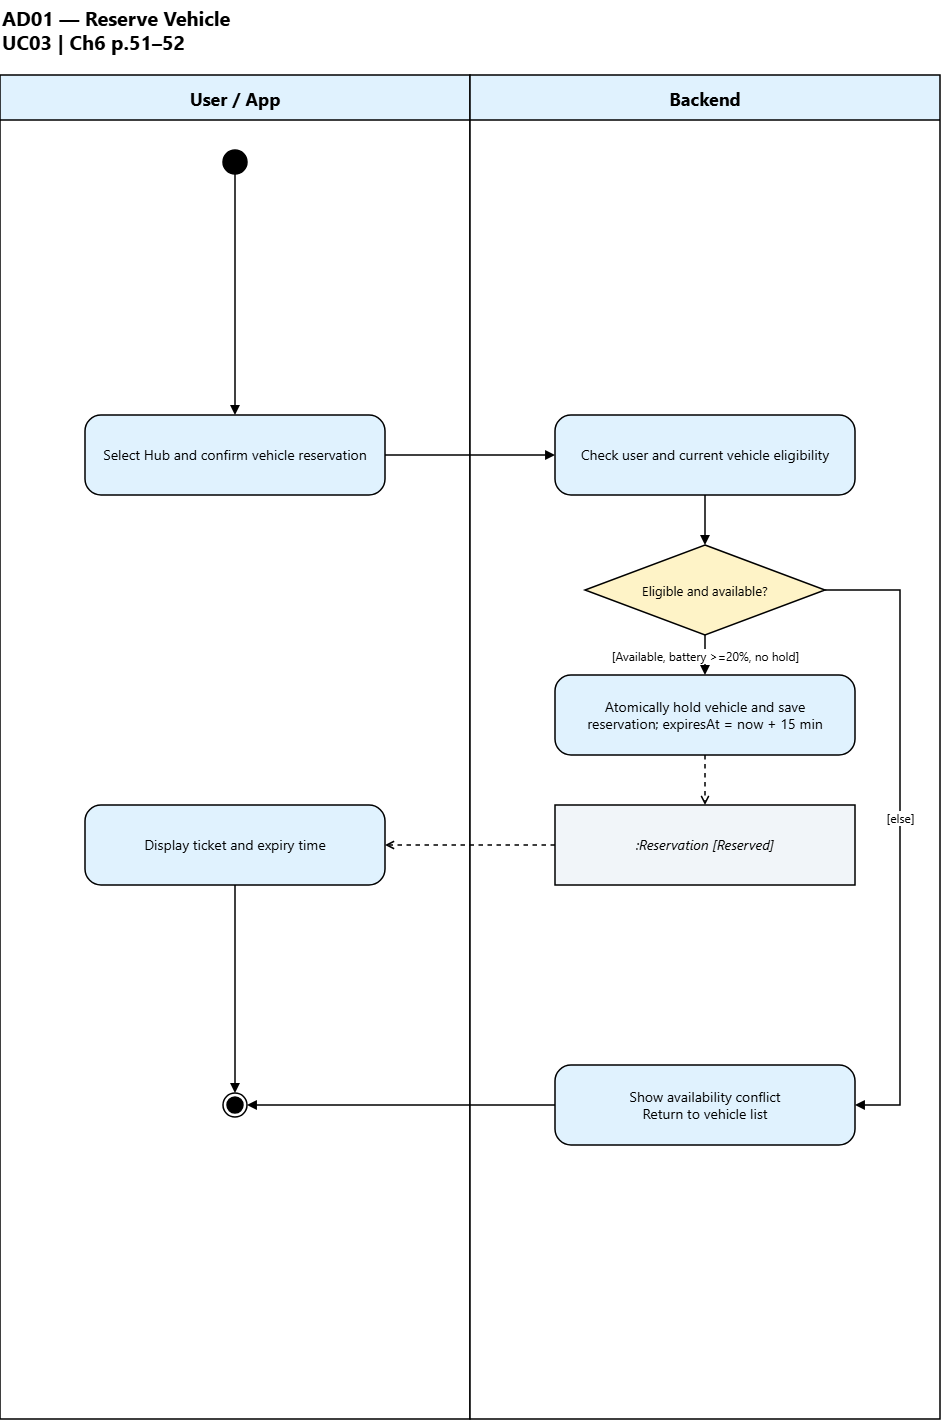
\includegraphics[width=0.95\textwidth,height=0.82\textheight,keepaspectratio]{graphics/diagrams/AD01-Reserve_Vehicle.png}
    \caption{Sơ đồ hoạt động đặt giữ xe dùng chung (\texttt{AD01 -- UC03})}
    \label{fig:ad-01}
\end{figure}

\clearpage
\begin{figure}[H]
    \centering
    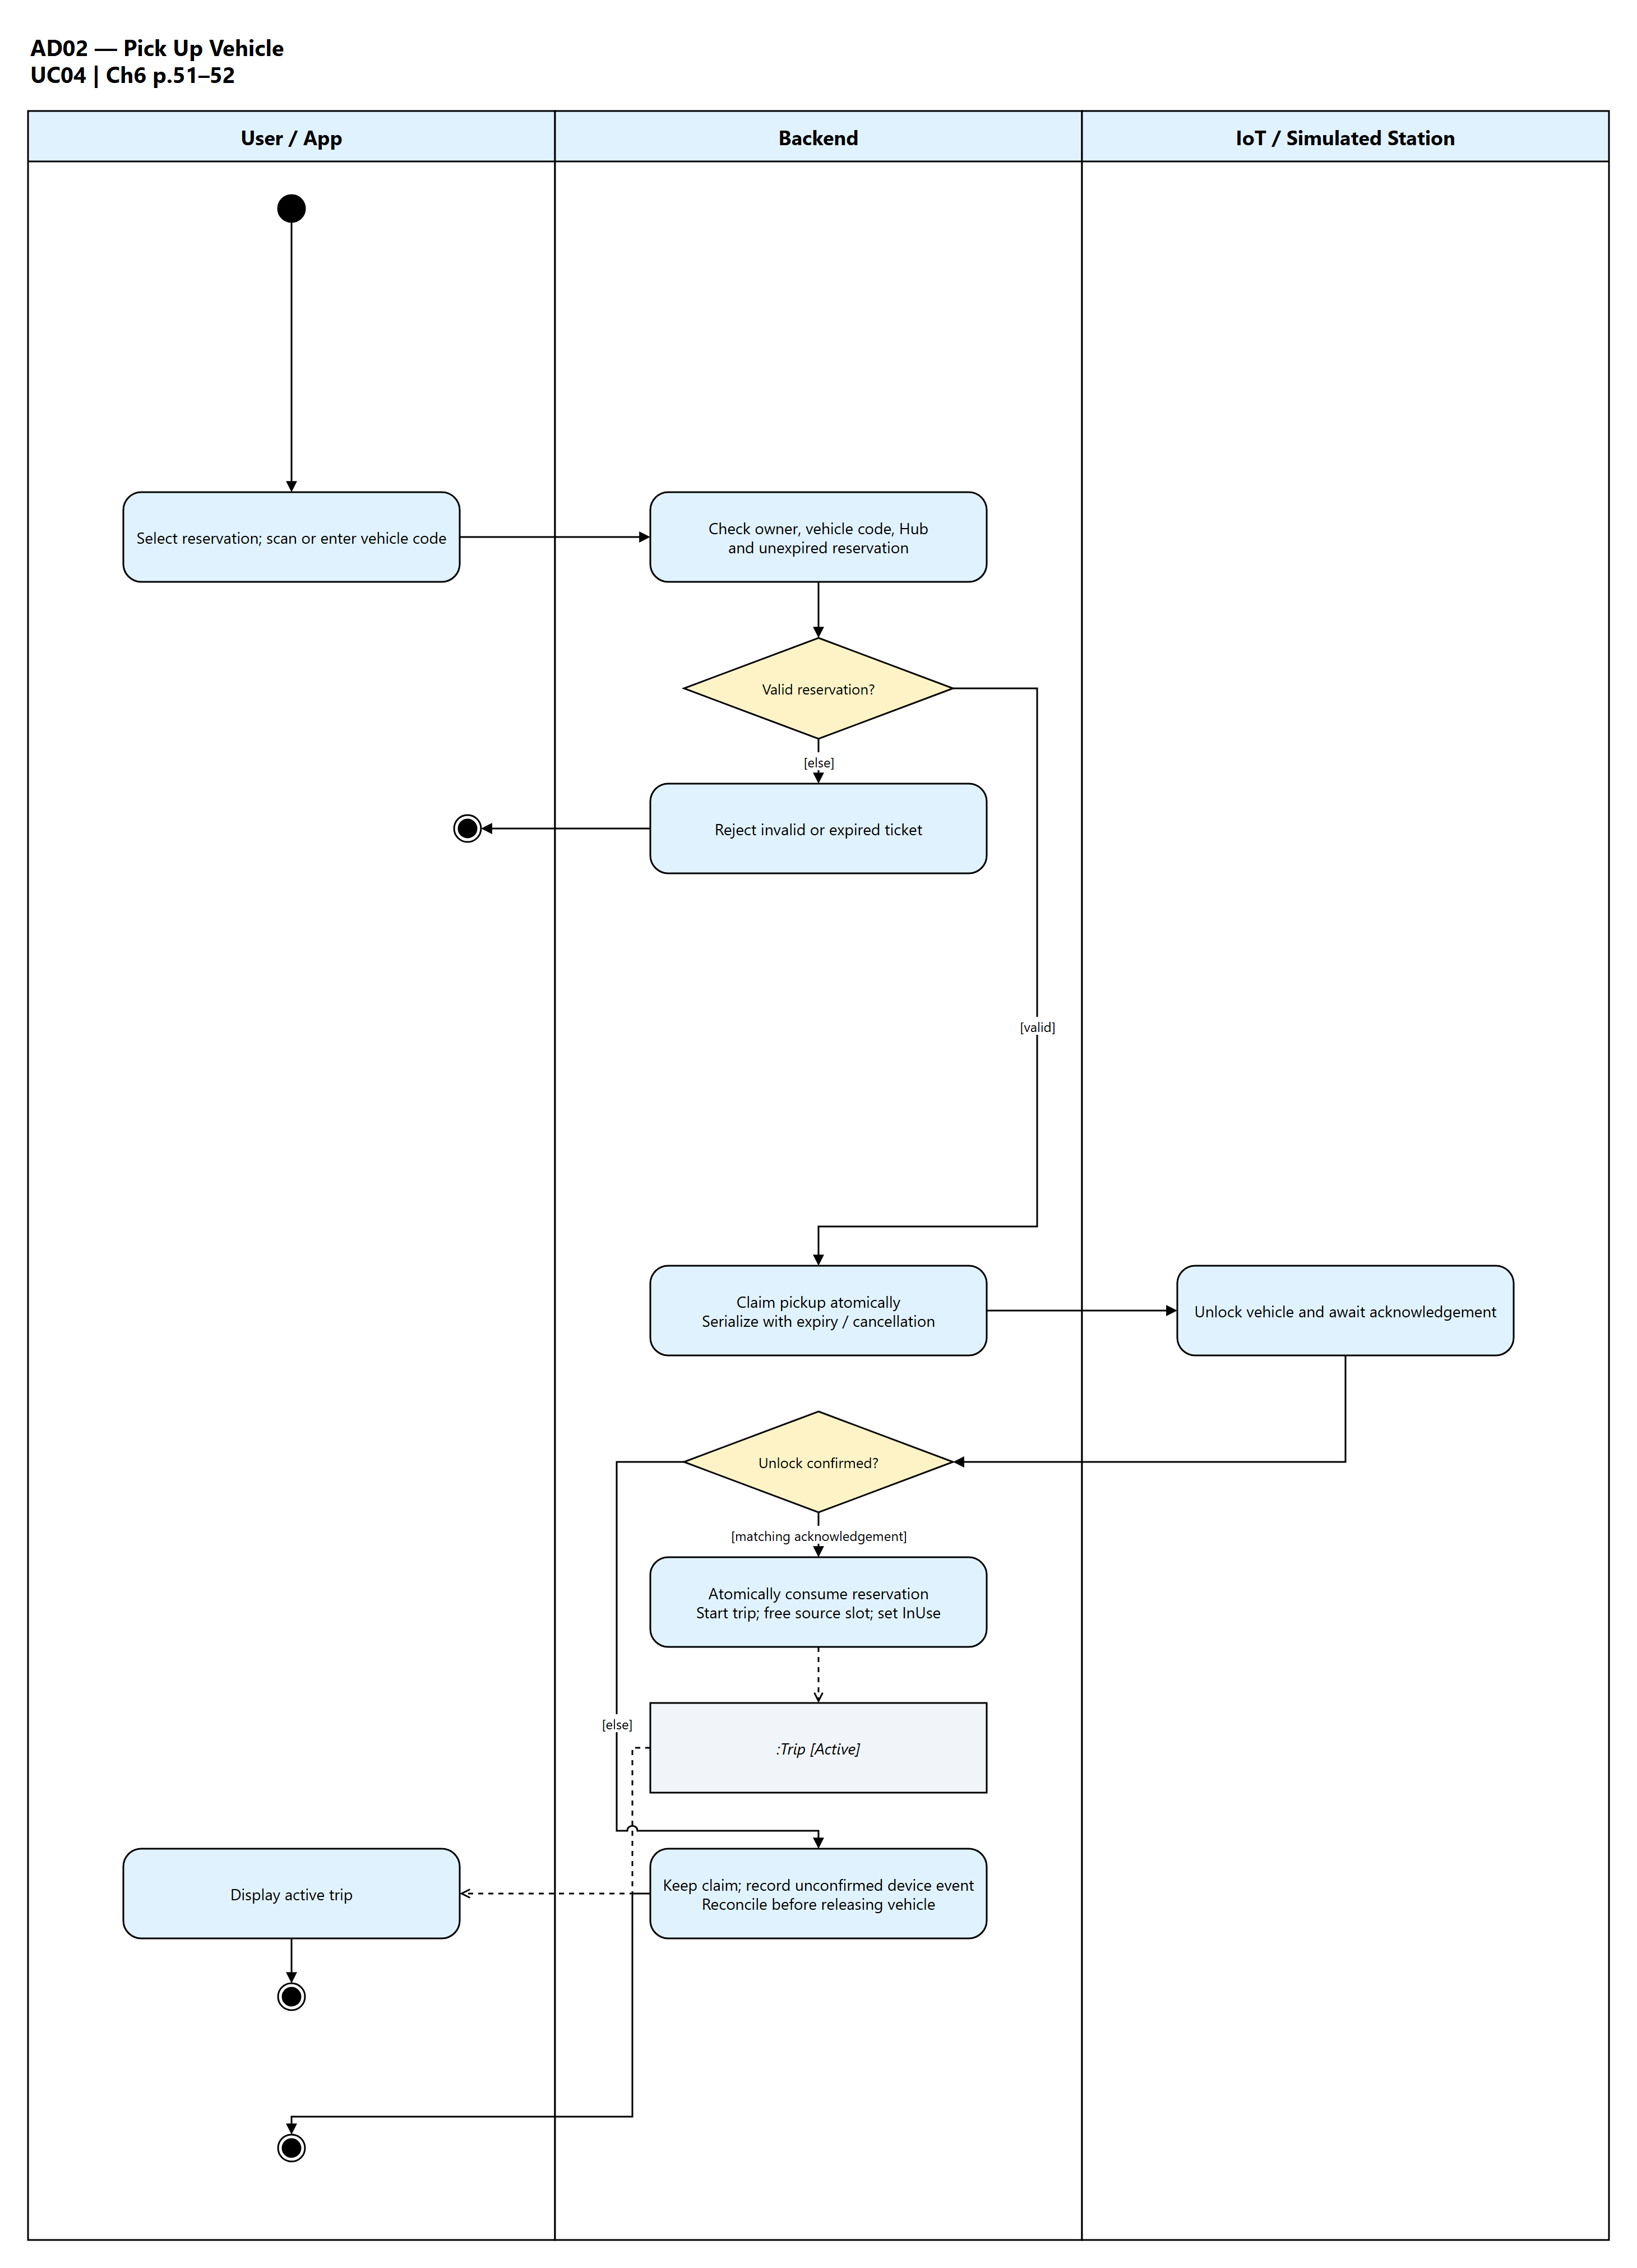
\includegraphics[width=0.95\textwidth,height=0.82\textheight,keepaspectratio]{graphics/diagrams/AD02-Pick_Up_Vehicle.png}
    \caption{Sơ đồ hoạt động nhận xe tại Hub (\texttt{AD02 -- UC04})}
    \label{fig:ad-02}
\end{figure}

\clearpage
\begin{figure}[H]
    \centering
    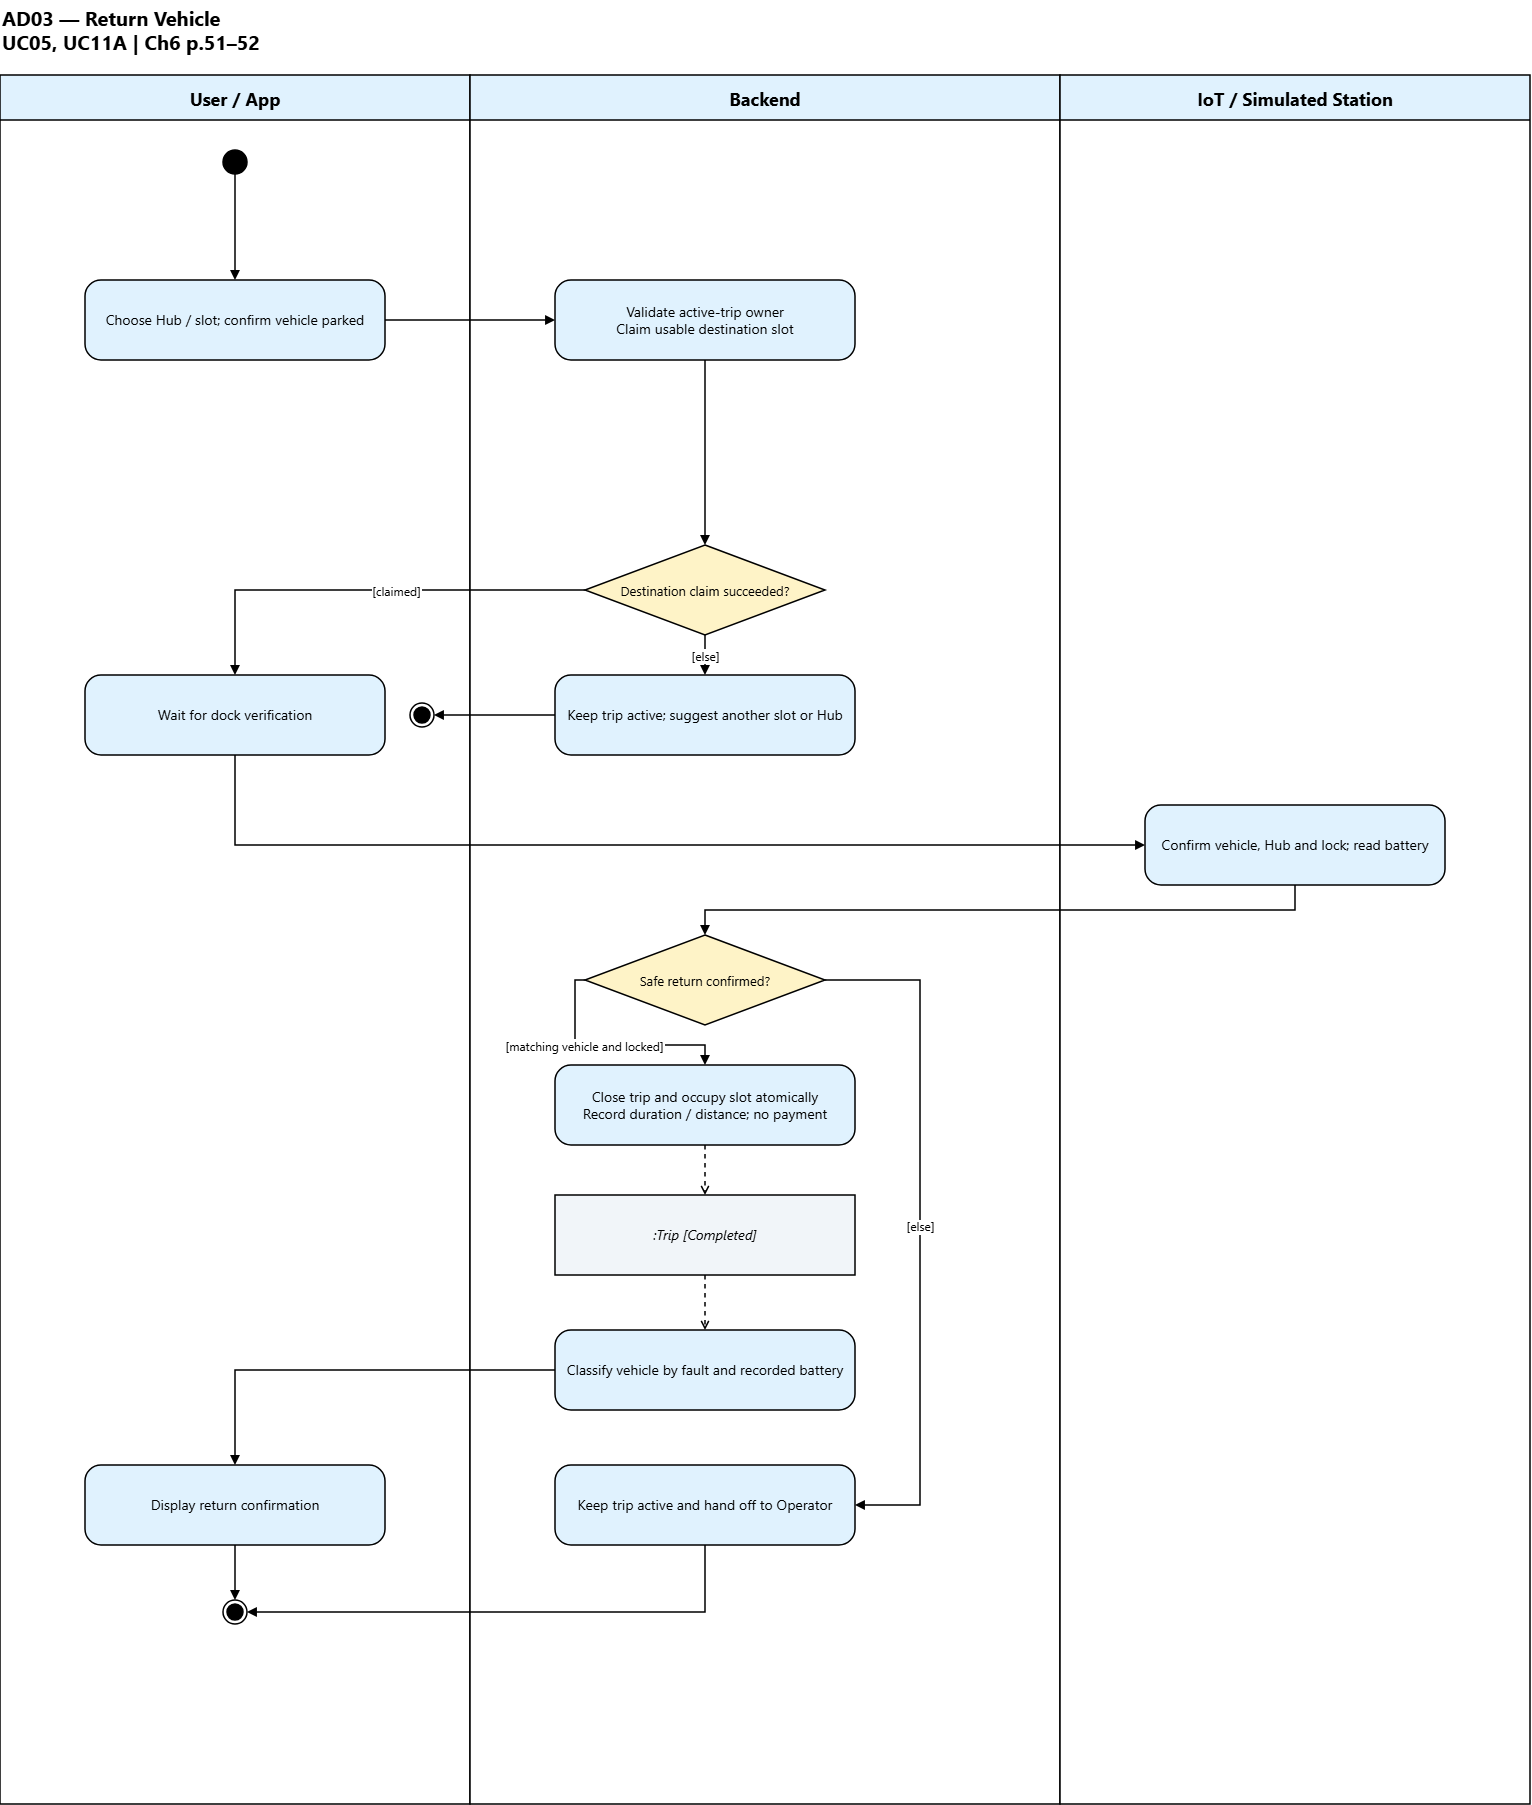
\includegraphics[width=0.95\textwidth,height=0.82\textheight,keepaspectratio]{graphics/diagrams/AD03-Return_Vehicle.png}
    \caption{Sơ đồ hoạt động trả xe tại Hub đích (\texttt{AD03 -- UC05})}
    \label{fig:ad-03}
\end{figure}

\clearpage
\begin{figure}[H]
    \centering
    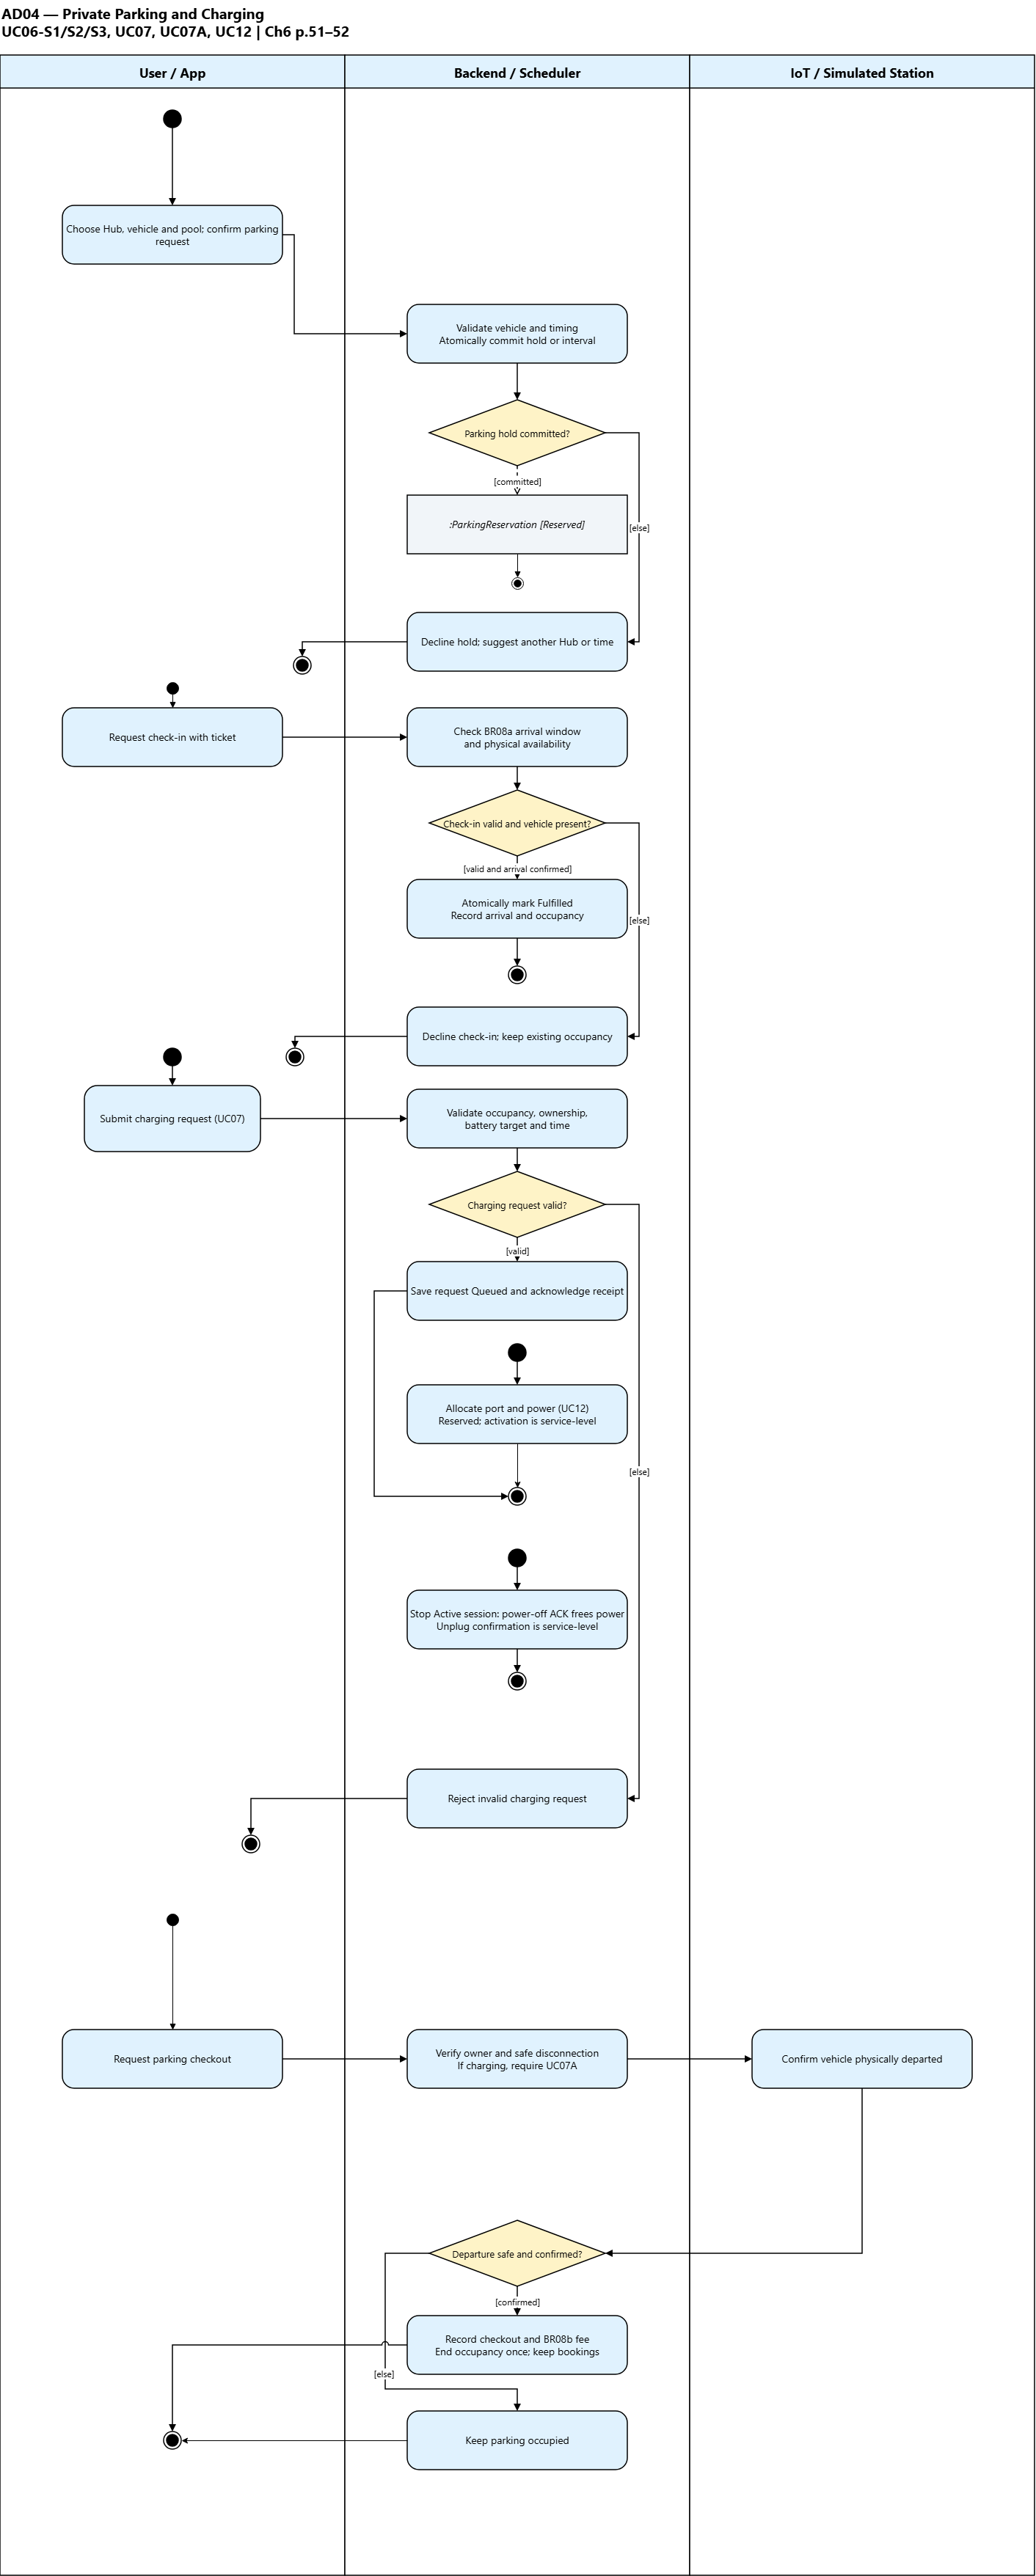
\includegraphics[width=0.95\textwidth,height=0.82\textheight,keepaspectratio]{graphics/diagrams/AD04-Reserve_Parking_and_Charging.png}
    \caption{Sơ đồ hoạt động đặt chỗ đỗ, sạc và dừng sạc xe cá nhân (\texttt{AD04 -- UC06, UC07, UC12})}
    \label{fig:ad-04}
\end{figure}

\clearpage
\begin{figure}[H]
    \centering
    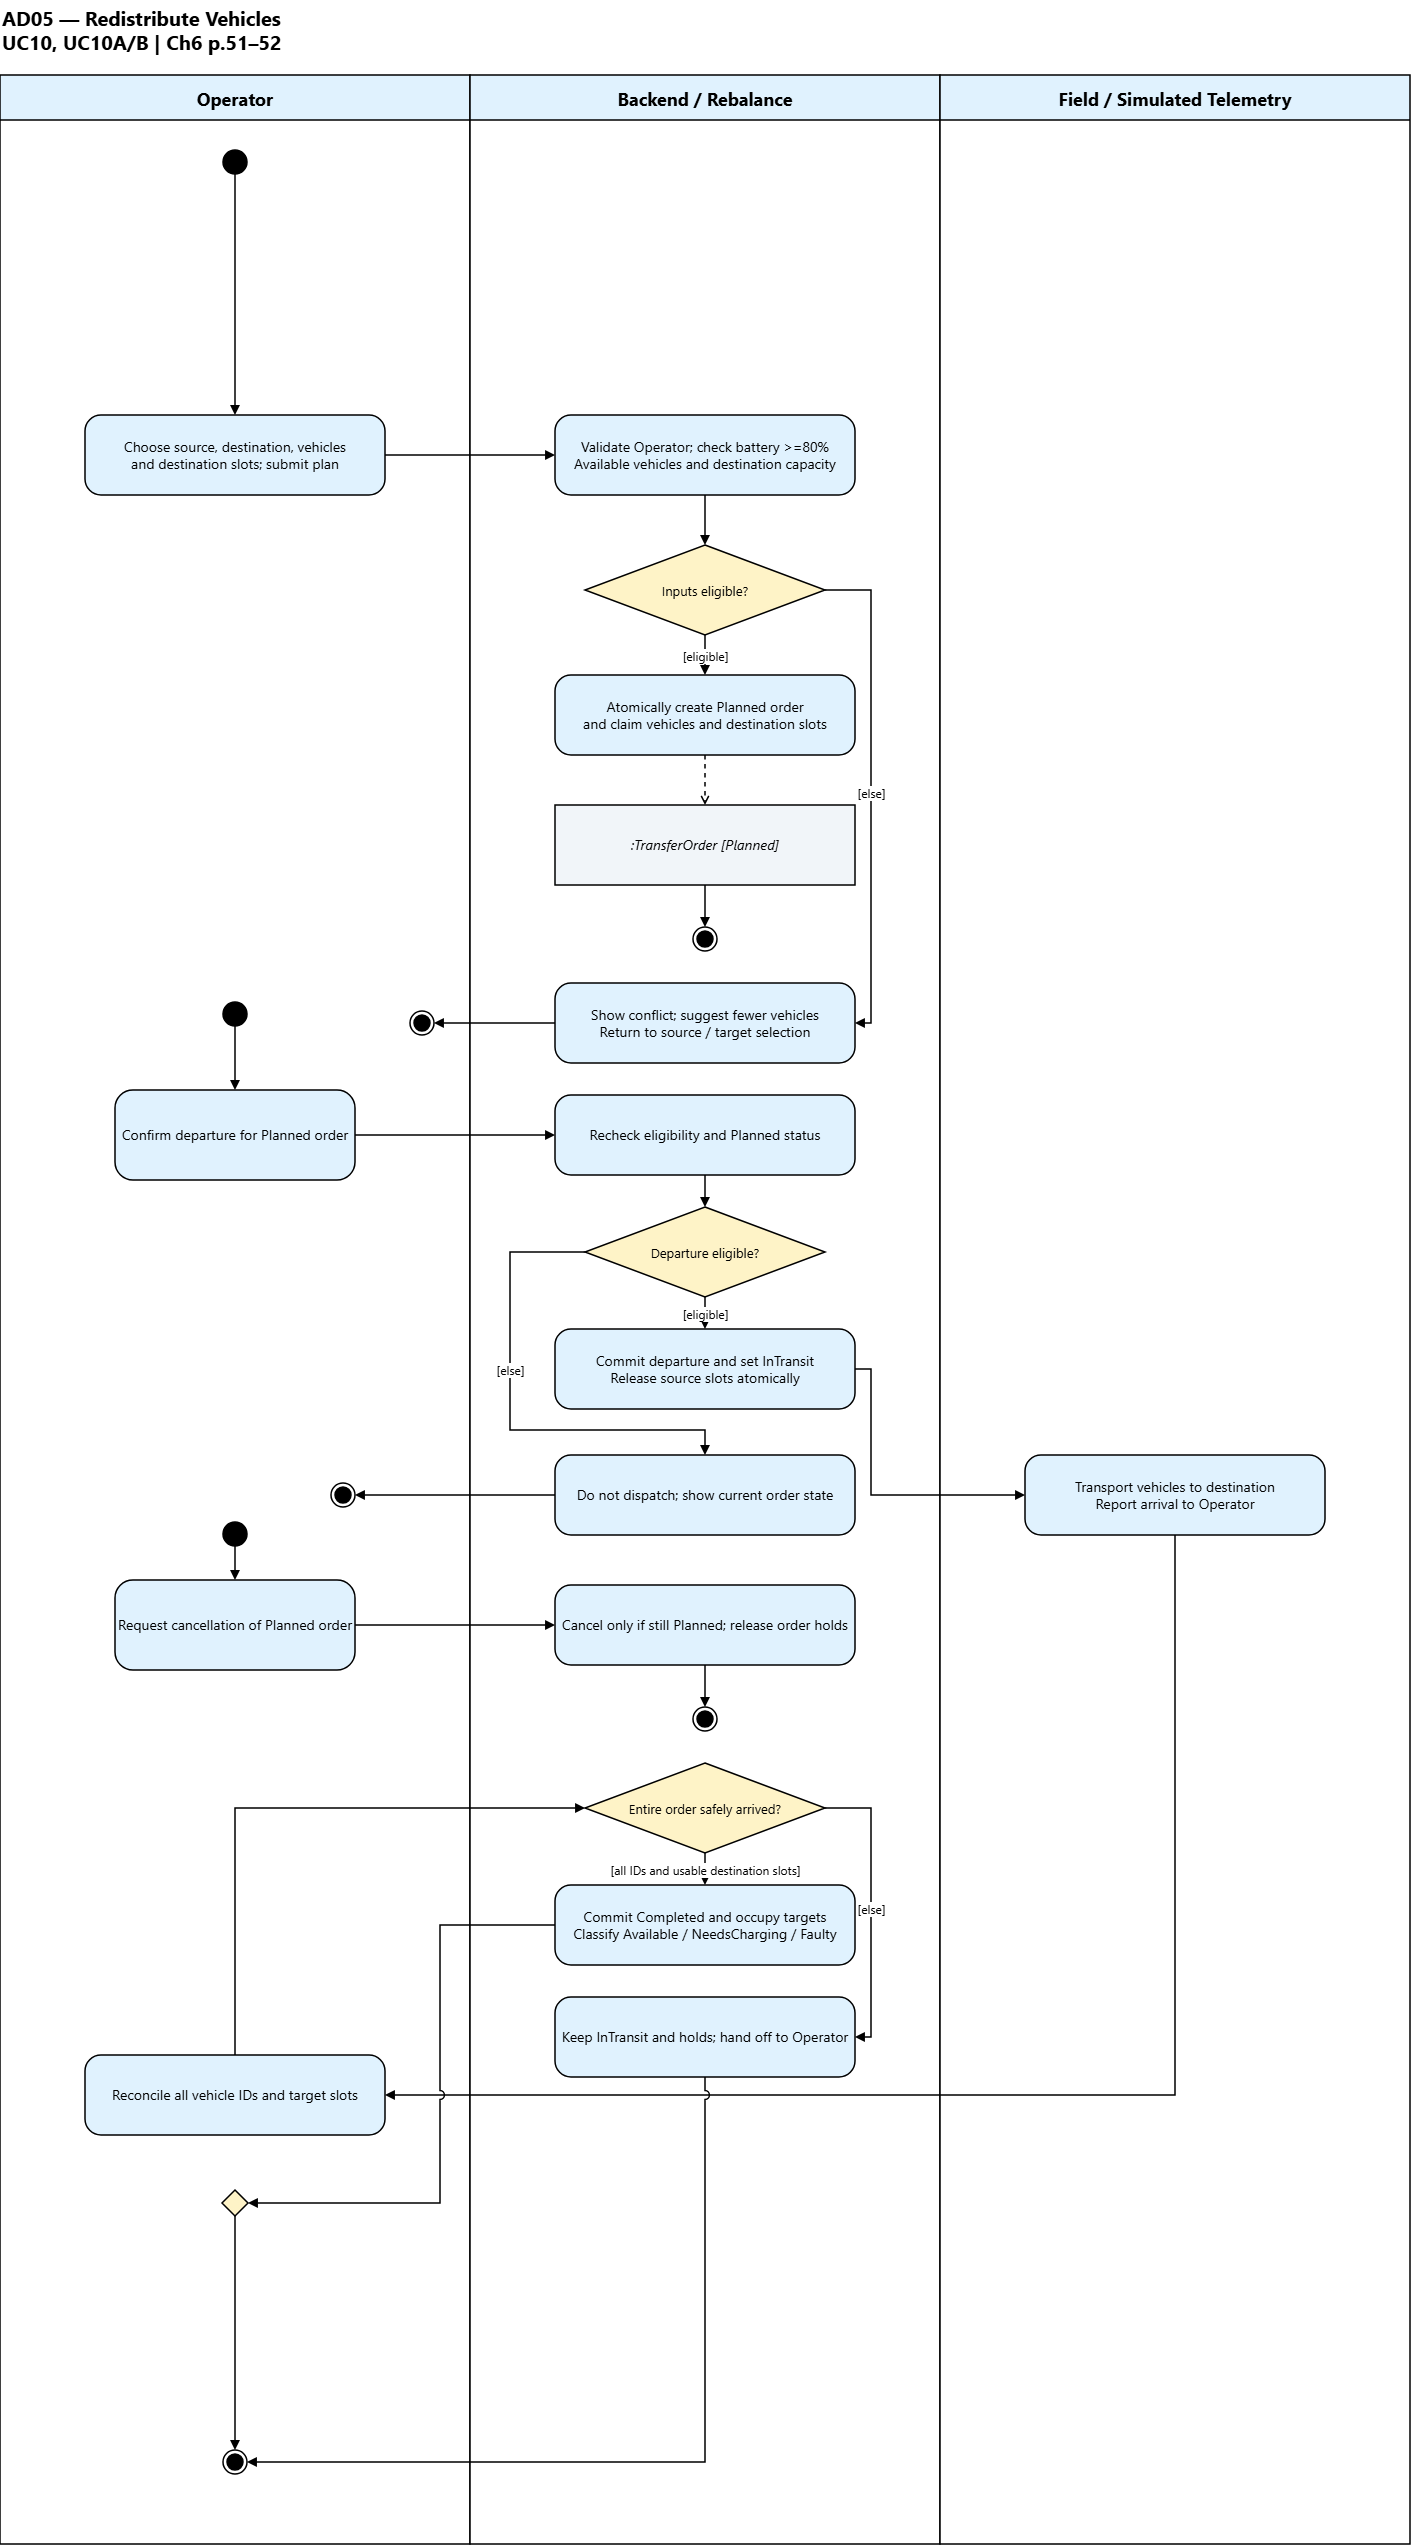
\includegraphics[width=0.95\textwidth,height=0.82\textheight,keepaspectratio]{graphics/diagrams/AD05-Redistribute_Vehicles.png}
    \caption{Sơ đồ hoạt động điều chuyển xe liên Hub (\texttt{AD05 -- UC10, UC10A/B})}
    \label{fig:ad-05}
\end{figure}

\clearpage
\begin{figure}[H]
    \centering
    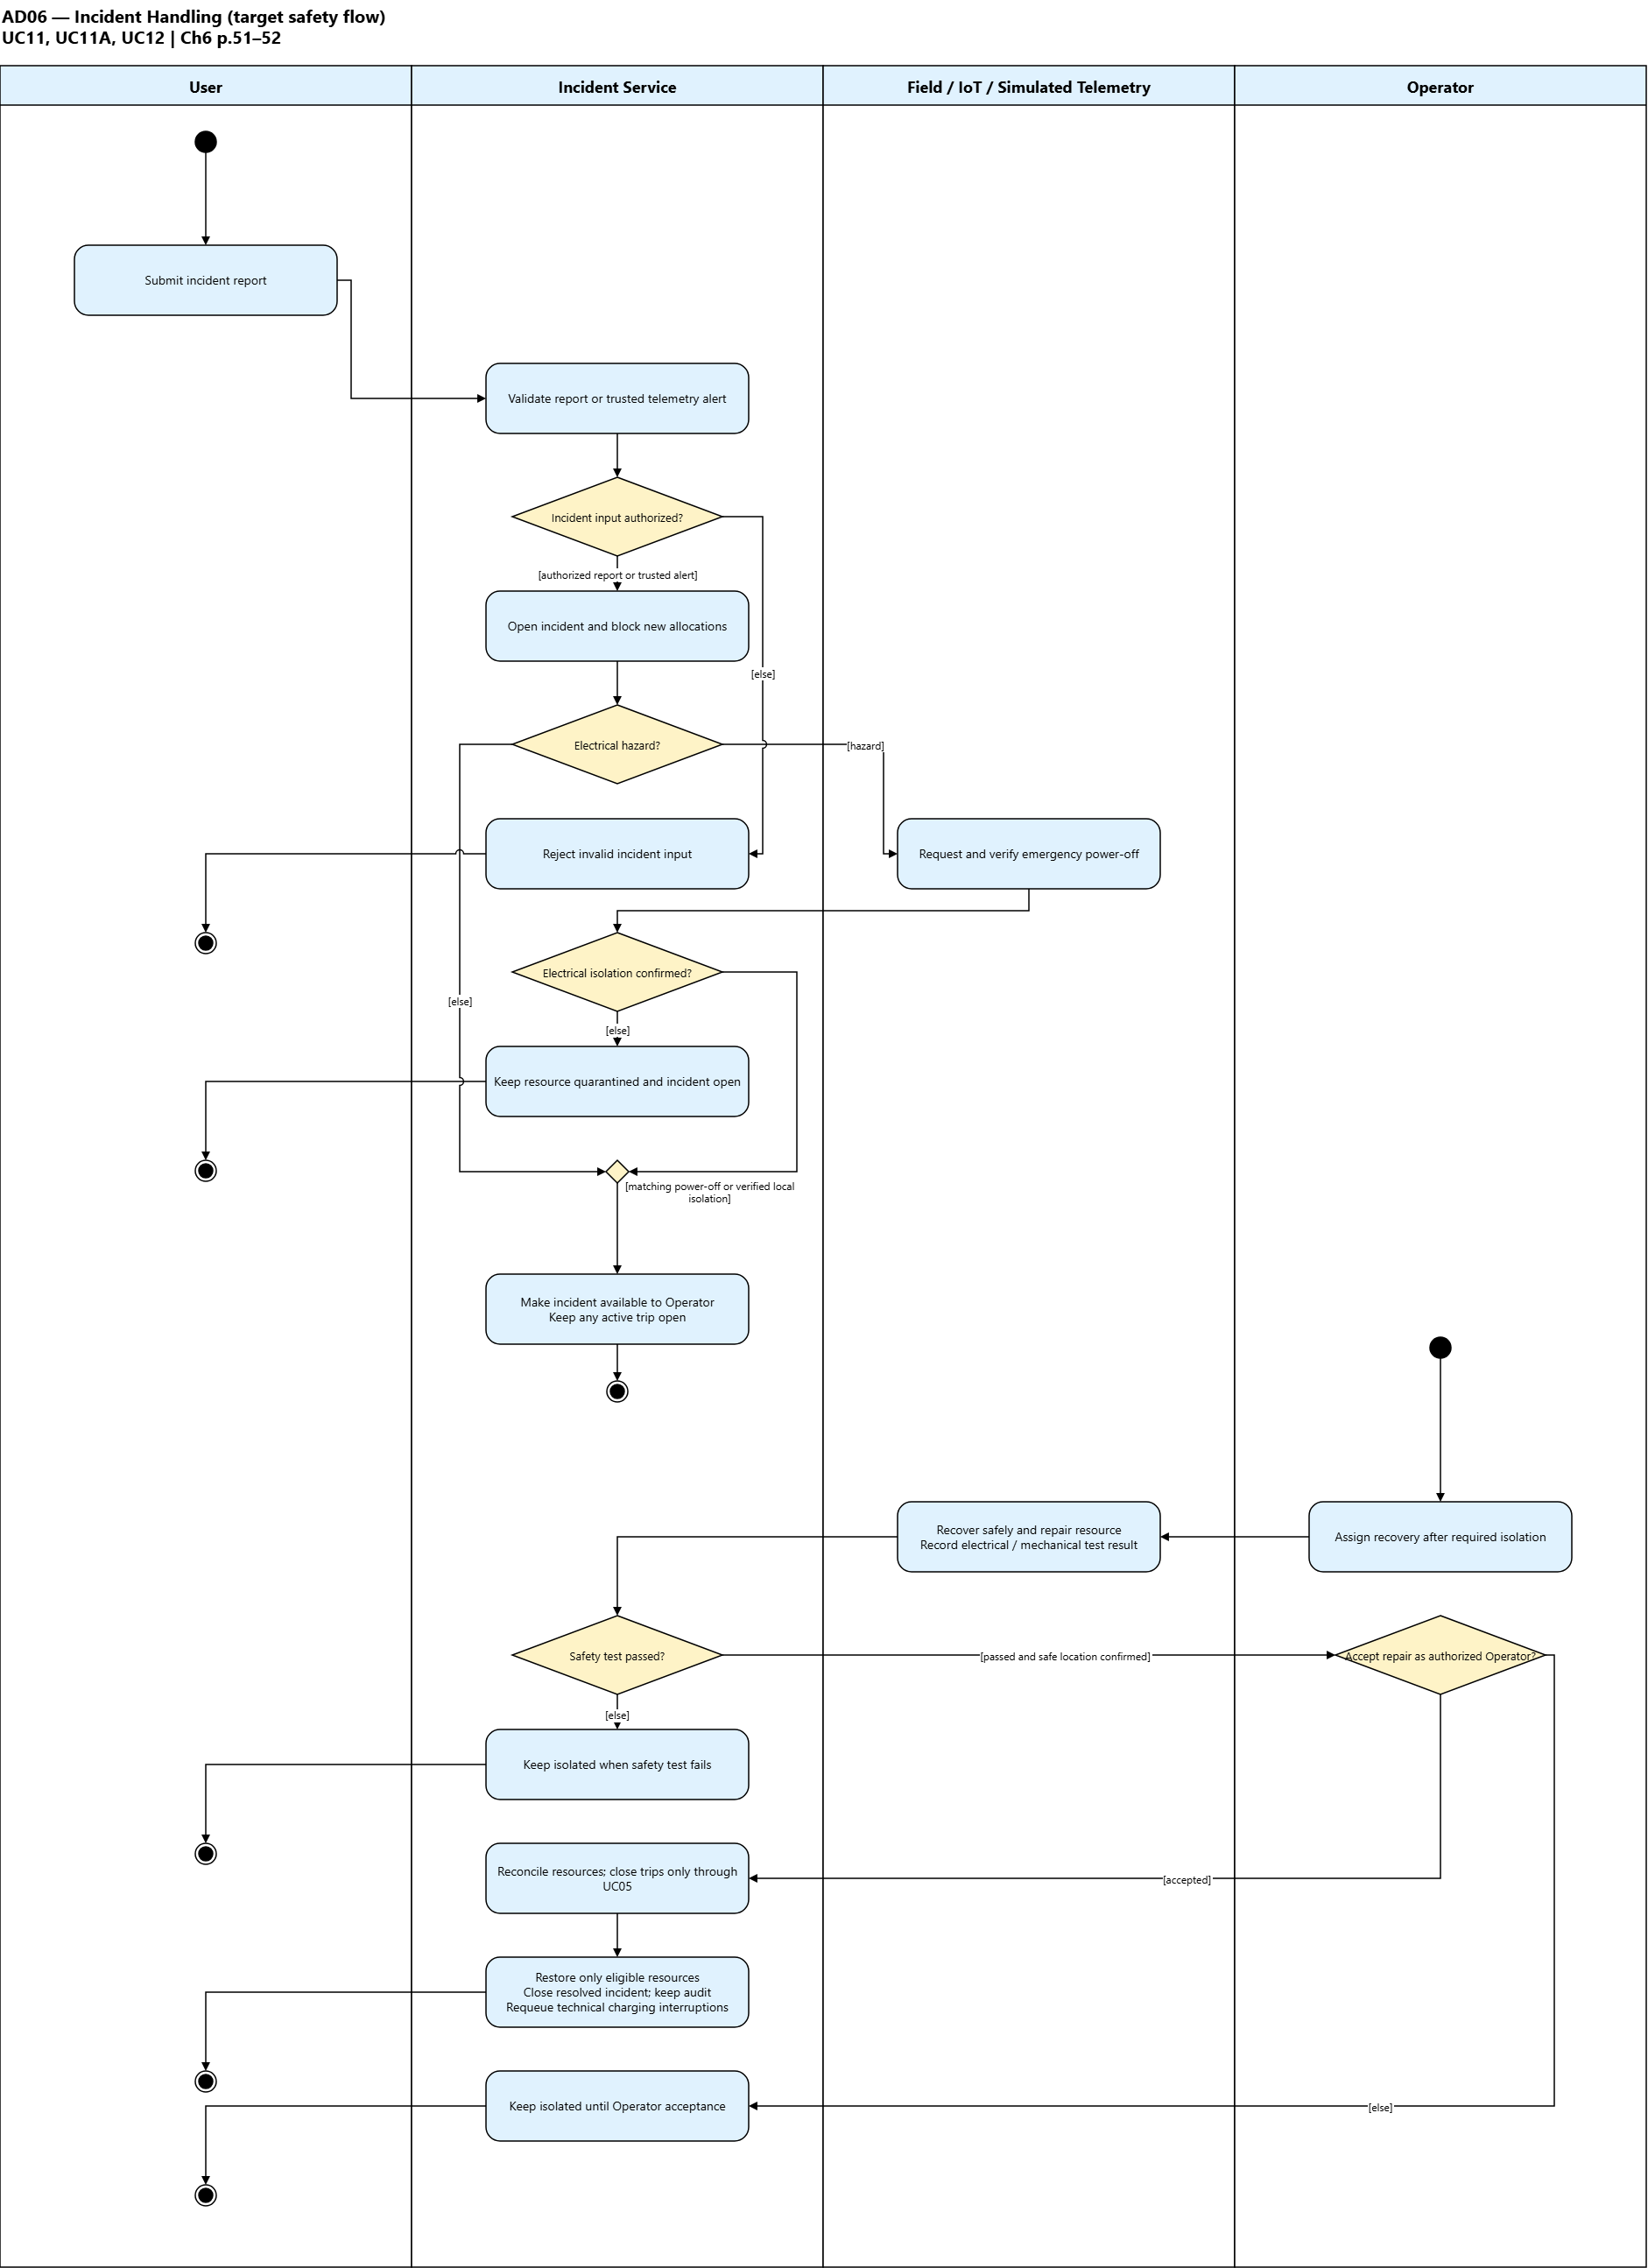
\includegraphics[width=0.95\textwidth,height=0.82\textheight,keepaspectratio]{graphics/diagrams/AD06-Handle_Operational_Incident.png}
    \caption{Sơ đồ hoạt động xử lý sự cố vận hành (\texttt{AD06 -- UC11, UC11A})}
    \label{fig:ad-06}
\end{figure}

\clearpage
\begin{figure}[H]
    \centering
    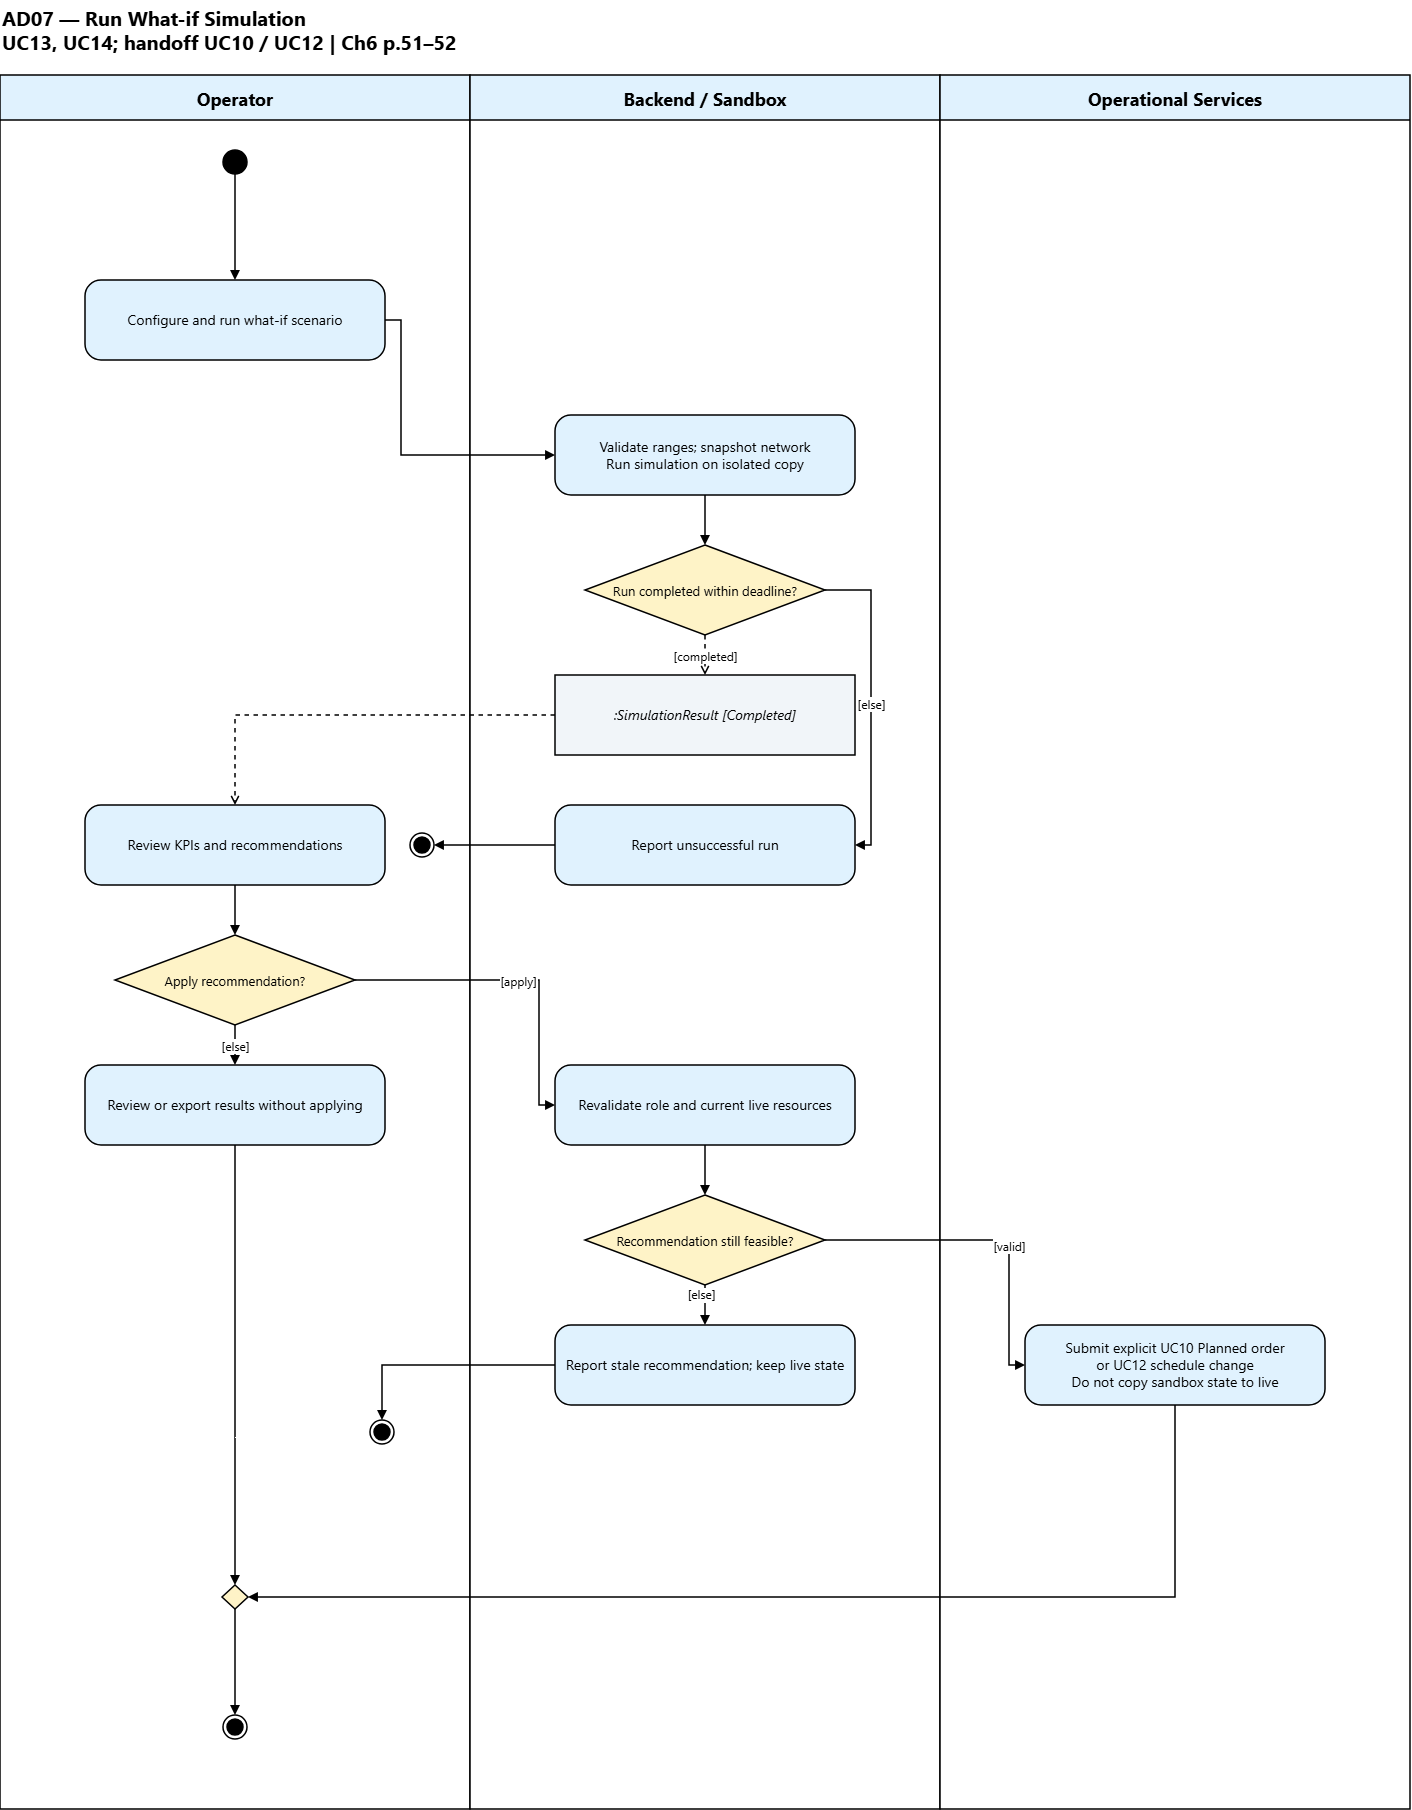
\includegraphics[width=0.95\textwidth,height=0.82\textheight,keepaspectratio]{graphics/diagrams/AD07-Run_What_if_Simulation.png}
    \caption{Sơ đồ hoạt động mô phỏng What-if (\texttt{AD07 -- UC13, UC14})}
    \label{fig:ad-07}
\end{figure}
\clearpage

\subsection{Mô hình Hành vi: Sơ đồ Trạng thái (State-chart Diagrams -- Bonus: SC01--SC03)}

Để đáp ứng tiêu chí điểm cộng của Submission \#2 và kiểm soát chuyển đổi trạng thái khi thực thi đồng thời, nhóm thiết kế 3 máy trạng thái hữu hạn cho các thực thể lõi (\Cref{fig:sc-01}--\Cref{fig:sc-03}):
\begin{enumerate}[leftmargin=*,nosep]
    \item \textbf{\texttt{SC01} -- Vòng đời Phương tiện Điện (\texttt{Vehicle State Machine}):} Mô hình hóa 10 trạng thái chuẩn (\texttt{Available}, \texttt{Reserved}, \texttt{InUse}, \texttt{Needs\allowbreak Charging}, \texttt{Charging}, \texttt{Transfer\allowbreak Held}, \texttt{InTransit}, \texttt{Faulty}, \texttt{Maintenance}, \texttt{Retired}). Điều kiện chuyển đổi phân biệt xe dùng chung (cho thuê và điều chuyển) với xe cá nhân (chỉ tham gia đỗ/sạc), đồng thời chặn chuyển về \texttt{Available} khi chưa nghiệm thu sự cố hoặc pin $< 20\%$.
    \item \textbf{\texttt{SC02} -- Vòng đời Cổng sạc (\texttt{Charging Point State Machine}):} Bao gồm 9 trạng thái (\texttt{Idle}, \texttt{Reserved}, \texttt{Starting}, \texttt{Charging}, \texttt{Stopping}, \texttt{Complete}, \texttt{Fault}, \texttt{Repair}, \texttt{Retired}), phân tách trạng thái \texttt{Complete} (đã ngắt điện, giữ đầu nối chờ rút) và duy trì khóa cô lập cổng \texttt{Fault/Repair}. Trong mã nguồn hiện tại, phần chuyển đổi từ \texttt{Reserved} sang \texttt{Active} (\texttt{activateAllocation}) và rút phích (\texttt{confirmUnplug}) được hiện thực ở tầng \texttt{ChargingService} kèm unit test, chưa mở route HTTP công khai.
    \item \textbf{\texttt{SC03} -- Vòng đời Đặt giữ và Chuyến đi (\texttt{Reservation and Trip State Machine}):} Quản lý song hành vòng đời phiếu giữ xe (\texttt{Pending}, \texttt{Reserved}, \texttt{Fulfilled}, \texttt{Cancelled}, \texttt{Expired}) với cờ \texttt{pickupClaimed} và vòng đời chuyến đi (\texttt{Active}, \texttt{Completed}). Sự cố báo giữa chuyến (\texttt{UC11A}) không tự động đóng chuyến đang \texttt{Active}.
\end{enumerate}

\clearpage
\begin{figure}[H]
    \centering
    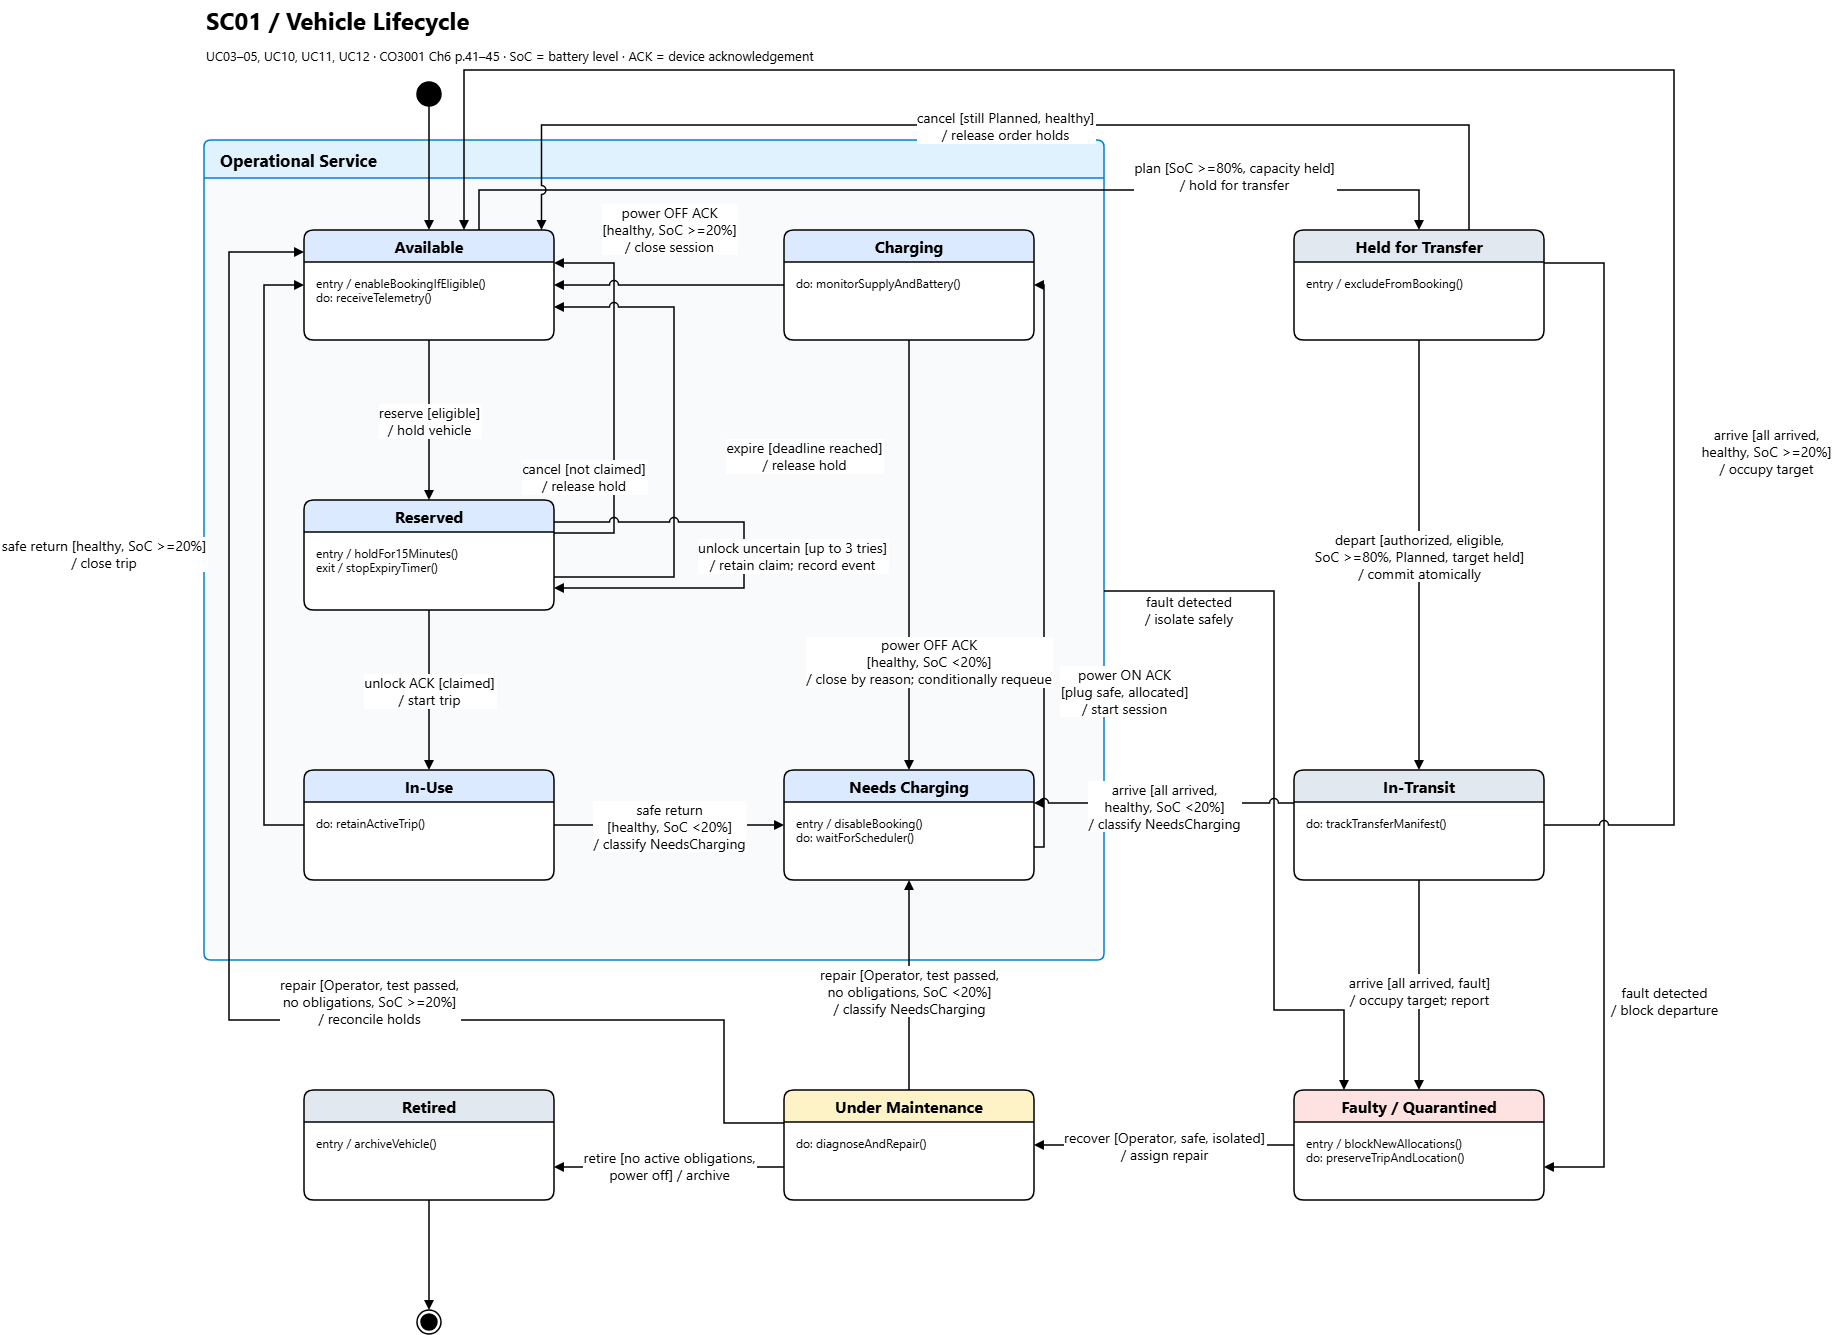
\includegraphics[width=0.95\textwidth,height=0.82\textheight,keepaspectratio]{graphics/diagrams/SC01-Vehicle_State_Machine.png}
    \caption{Sơ đồ máy trạng thái vòng đời phương tiện điện (\texttt{SC01})}
    \label{fig:sc-01}
\end{figure}

\clearpage
\begin{figure}[H]
    \centering
    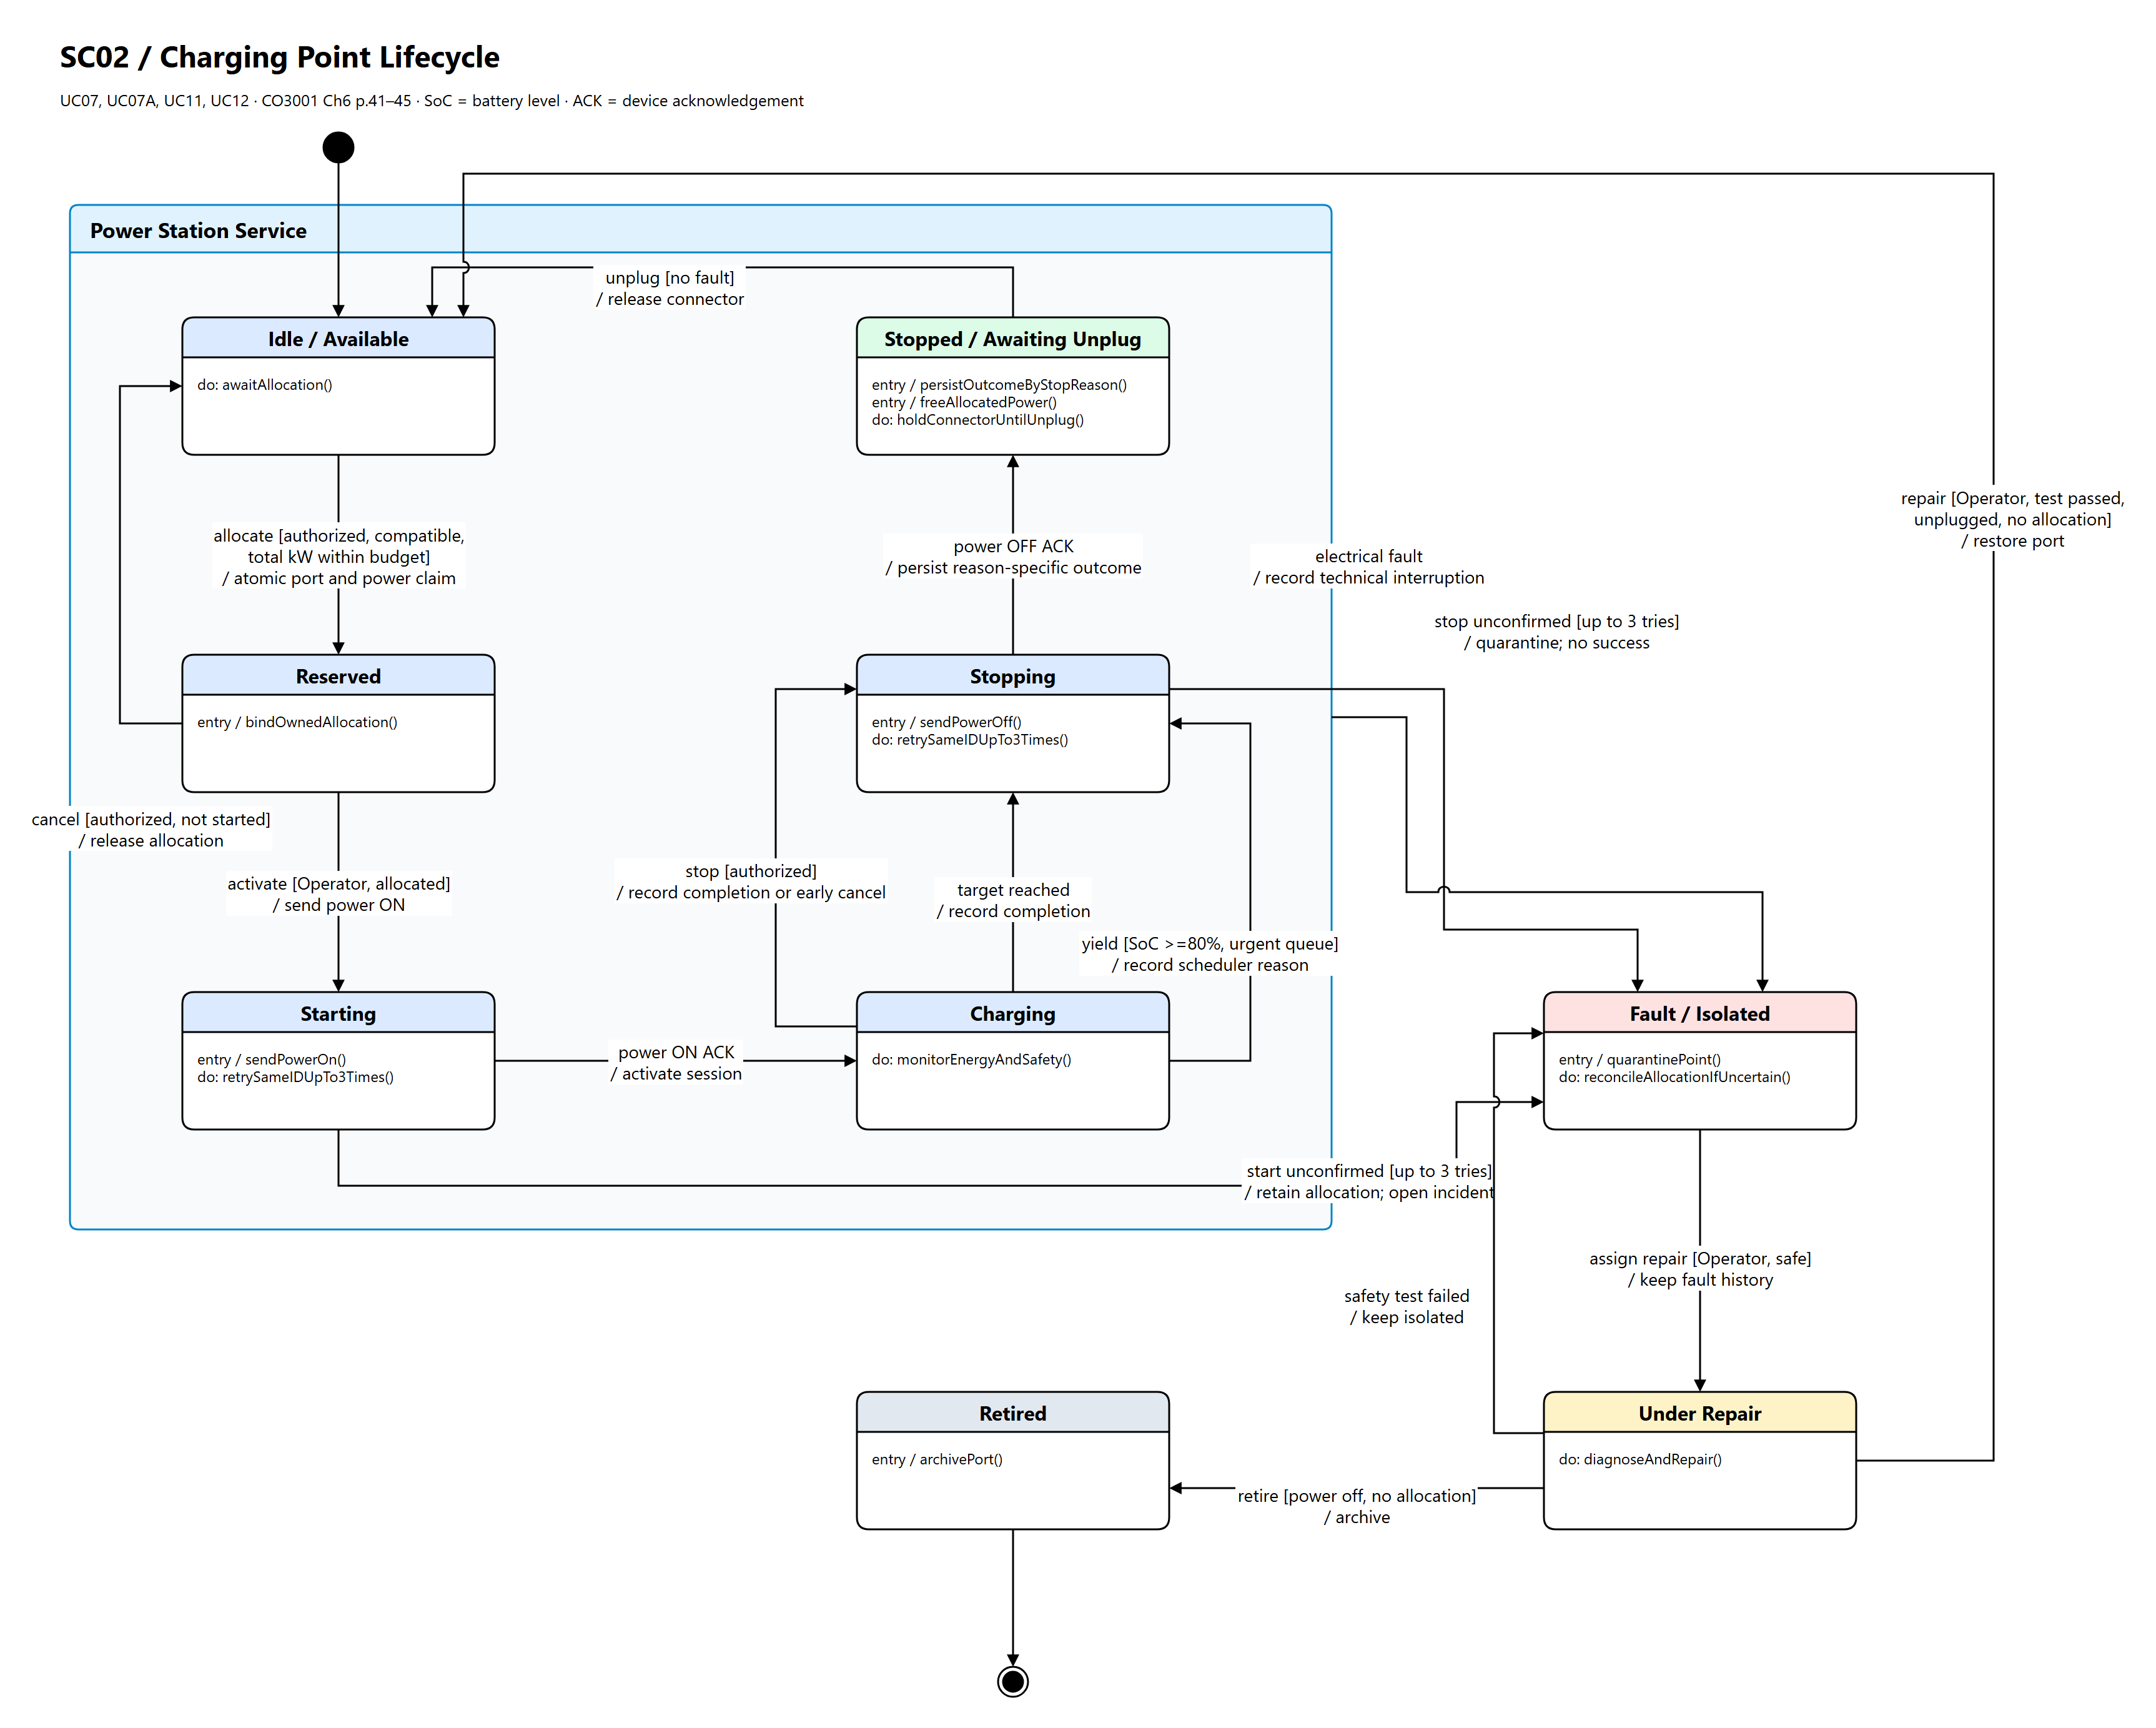
\includegraphics[width=0.95\textwidth,height=0.82\textheight,keepaspectratio]{graphics/diagrams/SC02-Charging_Point_State_Machine.png}
    \caption{Sơ đồ máy trạng thái vòng đời cổng sạc (\texttt{SC02})}
    \label{fig:sc-02}
\end{figure}

\clearpage
\begin{figure}[H]
    \centering
    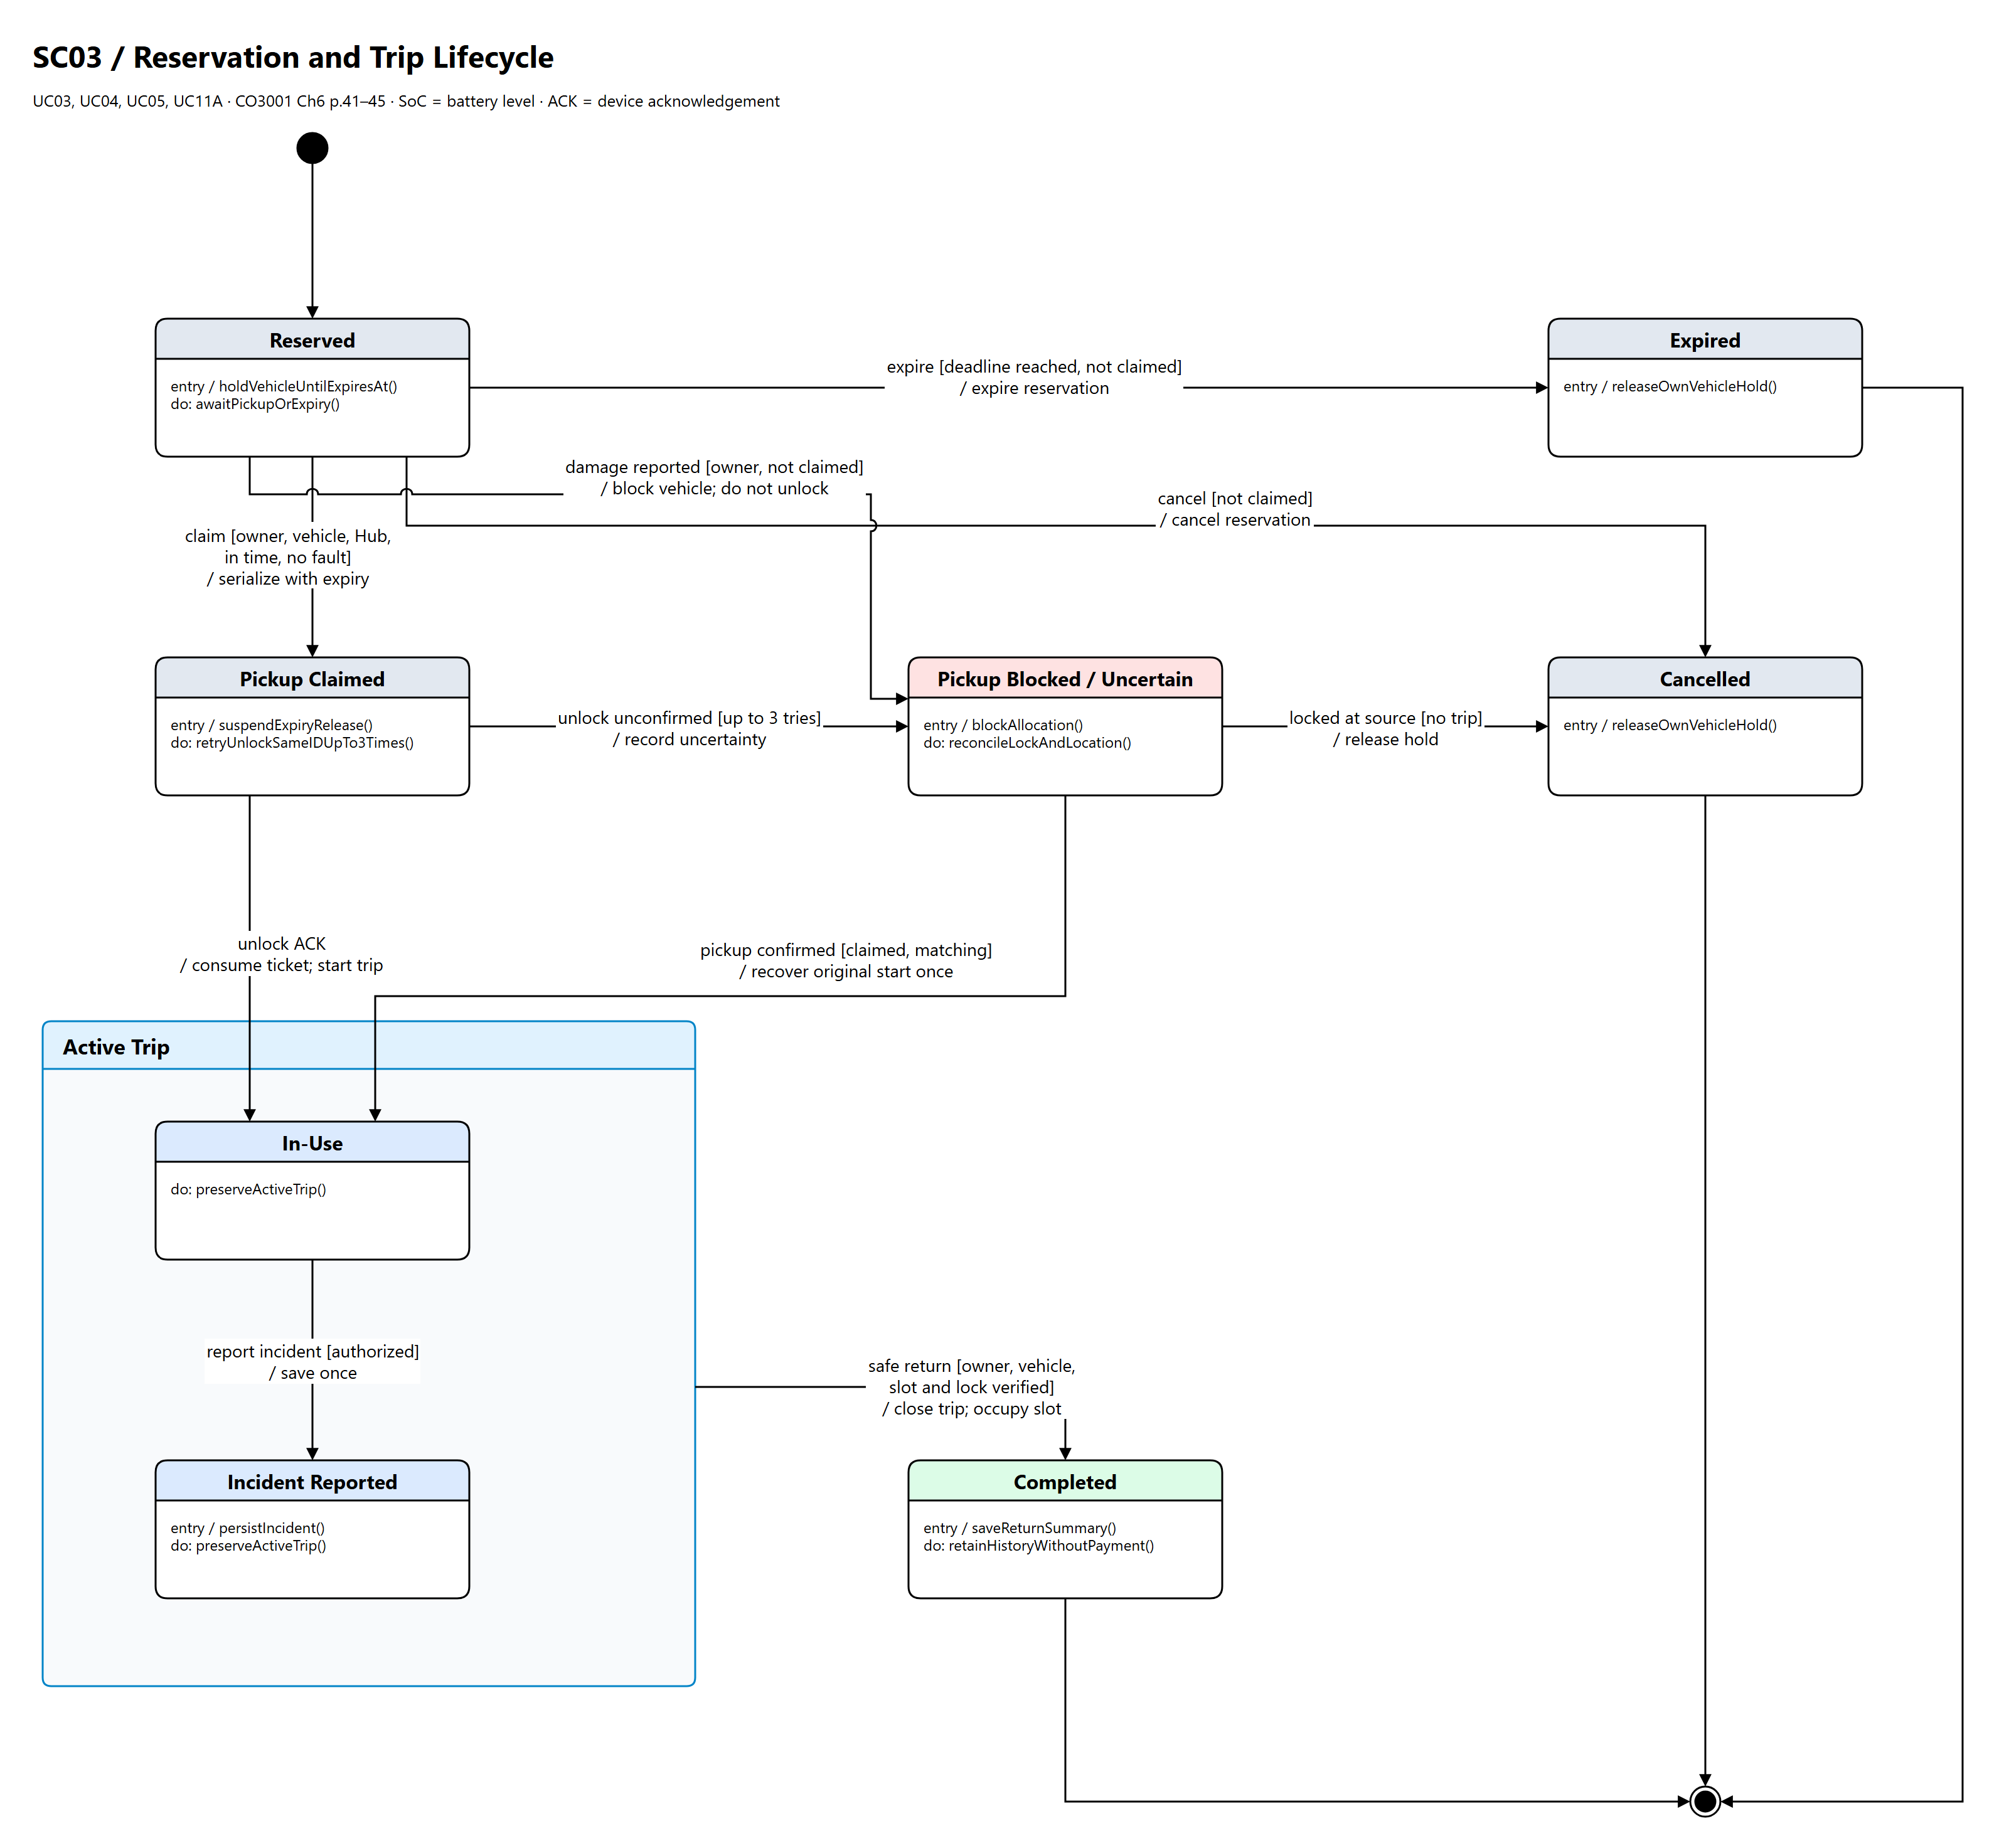
\includegraphics[width=0.95\textwidth,height=0.82\textheight,keepaspectratio]{graphics/diagrams/SC03-Reservation_and_Trip_State_Machine.png}
    \caption{Sơ đồ máy trạng thái đặt giữ và chuyến đi (\texttt{SC03})}
    \label{fig:sc-03}
\end{figure}
